\newpage
% \section{Overleaf 使用注意事项}

% 如果你在Overleaf上编译本模板,请注意如下事项~\cite{zjuthesis}:

% \begin{itemize}
%     \item 删除根目录的 ``.latexmkrc'' 文件,否则编译失败且不报任何错误
%     \item 字体有版权所以本模板不能附带字体,请务必手动上传字体文件,并在各个专业模板下手动指定字体。
%         具体方法参照 GitHub 主页的说明。
%     \item 当前(2019年9月2日)的Overleaf使用TexLive 2017进行编译,但一些伪粗体复制乱码的问题需要TexLive 2019版本来解决。
%         所以各位同学可以在Overleaf上编写论文,但务必使用本地的TexLive 2019来进行最终编译,以免产生查重相关问题。
%         具体说明参照 GitHub 主页。
% \end{itemize}
\section{背景知识和相关技术}
\subsection{扩散模型}
\subsubsection{扩散模型的应用及研究意义}
\par
扩散模型因其独特的工作机制,在文生图、图生图等视觉内容生成方面展现了显著的优势。首先,扩
散模型能够生成非常逼真并且细节丰富的图像,其次,扩散模型具有较强的稳定性和可靠性,
通过基于概率的方法来有效地避免训练不稳定的问题,而这些问题在其他类型的
生成模型中较为常见\cite{ho2020denoising, rombach2022high}。相较于传统生成对抗网络(GAN)和变分自编码器(VAE),扩散模
型在生成质量与训练稳定性间取得了显著平衡\cite{sohl2015deep, dhariwal2021diffusion},在艺术创作、图像编辑、视频生成等
领域具有广泛应用前景。
\par
在应用层面,扩散模型正向多学科交叉领域延伸。时空扩散架构为地震预测、疾病控制
和城市规划等领域带来更准确的分析和预测能力,在性能上显著超越现有解决方案,平均提
升幅度超过50\%\cite{ruhling2023dyffusion, yuan2023spatio};
在生物学中,三维扩散框架在生成分子的成功率上比传统方法提升了三倍\cite{peng2023moldiff},
同时生成分子的质量更高;在跨模态生成方面,层级化扩散模型通过实现了文本-图像-视
频的连贯内容创作\cite{yang2024cross},提供了更高质量的动态内容生成系统。因此,扩散模型在处理复杂系统
不确定性方面具有独特意义及研究价值。
\subsubsection{扩散模型的原理}
\par
扩散模型的核心思想是通过逐步去除高斯噪声来生成以文本为条件的图像等视觉内容,
整体运行分为两个主要阶段:{\bfseries 前向扩散阶段}和{\bfseries 去噪推理阶段}。
这两个阶段共同构成了扩散模型的完整工作框架,并通过马尔卡夫链与深度学习相结合,
最终实现从原始噪声到复杂数据的稳定高效生成\cite{ho2020denoising}。
\par
在前向扩散阶段,原始图像通过马尔可夫链逐步添加高斯噪声,
最终使原始图像转化为纯随机噪声。
这一过程将复杂的原始数据逐步转化为标准高斯分布,为后续的去噪推理阶段提供转化来源。
其中,主要使用到以下两个机制:
\begin{itemize}
    \item {\bfseries 马尔可夫链特性:}马尔可夫链保证了
    前向扩散过程每一步的状态$x_{t}$只依赖于前一状态 $x_{t-1}$,与之前的状态信息无关,
    确保了前向扩散过程可以被反向传播,同时保证反向传播的计算比较简单,推理效率较高\cite{Zekri2024LargeLM}。
    \item {\bfseries 噪声添加机制:}每一步的噪声添加使用一个预定义的噪声调度器进行处理,
    使用如下公式进行噪声的添加\cite{ho2020denoising}:
    \begin{equation}
    q(x_t | x_{t-1}) = \mathcal{N}(x_t; \sqrt{1-\beta_t} x_{t-1}, \beta_t I)
    \end{equation}
    其中,$\beta_t$ 是第 $t$ 步的噪声系数。随着步骤的增加,$x_{t}$前的整体系数在不断相乘中
    逐步变小,因此噪声的占比不断扩大,
    原始数据逐渐被噪声覆盖,最终在 $T$ 步时完全变为符合高斯分布的纯噪声,即
    $x_T \sim \mathcal{N}(0, I)$。
\end{itemize}
\par
在去噪推理阶段,主要目标是从纯噪声 $x_T$ 出发,通过逐步预测噪声并去除对应噪声,
最终恢复出对应的图像。这一过程本质上是前向扩散的逆操作。主要步骤如下:
\begin{itemize}
    \item {\bfseries 噪声预测与去除:}在去噪推理分每一步中,模型根据当前噪声状态 $x_t$ 
    和时间步 $t$,预测当前需要添加的噪声 $\epsilon_\theta(x_t, t)$,然后将噪声从当前状态中
    去除,从而逐步去噪恢复数据特征。使用如下公式进行噪声的预测\cite{ho2020denoising}:
    \begin{equation}
        p_\theta(x_{t-1} | x_t) = \mathcal{N}(x_{t-1}; \mu_\theta(x_t, t), \Sigma_\theta(x_t, t))
    \end{equation}
    其中,$\mu_\theta$ 为均值预测参数, $\Sigma_\theta$ 为方差的预测参数,可以通过
    神经网络训练得到。
    \item {\bfseries 文本等输入控制:}去噪推理过程中的每一步实际调整较小。
    可以通过文本等输入在后续步骤中不断控制噪声的生成。例如:在文本生成图像的任务中,
    模型会结合文本的嵌入向量(如使用CLIP模型得到的语义向量)逐步指导去噪过程,
    确保生成结果与输入文本具有更高的一致性\cite{rombach2022high, Radford2021LearningTV, Liu2024TowardsUC}。
\end{itemize}
\subsubsection{典型扩散模型的具体架构}
\par
目前,典型的扩散模型(如:SDXL文生图模型)主要使用U-Net模型作为去噪推理过程的噪声预测模型,
它也是扩散模型最核心的结构,其余部分主要用于文本、图像等数据的编码、解码等过程,与本文研究内容无关,
这里不再赘述,具体架构如\autoref{fig:stable_diffusion}所示:
\begin{figure}[ht]
    \centering
    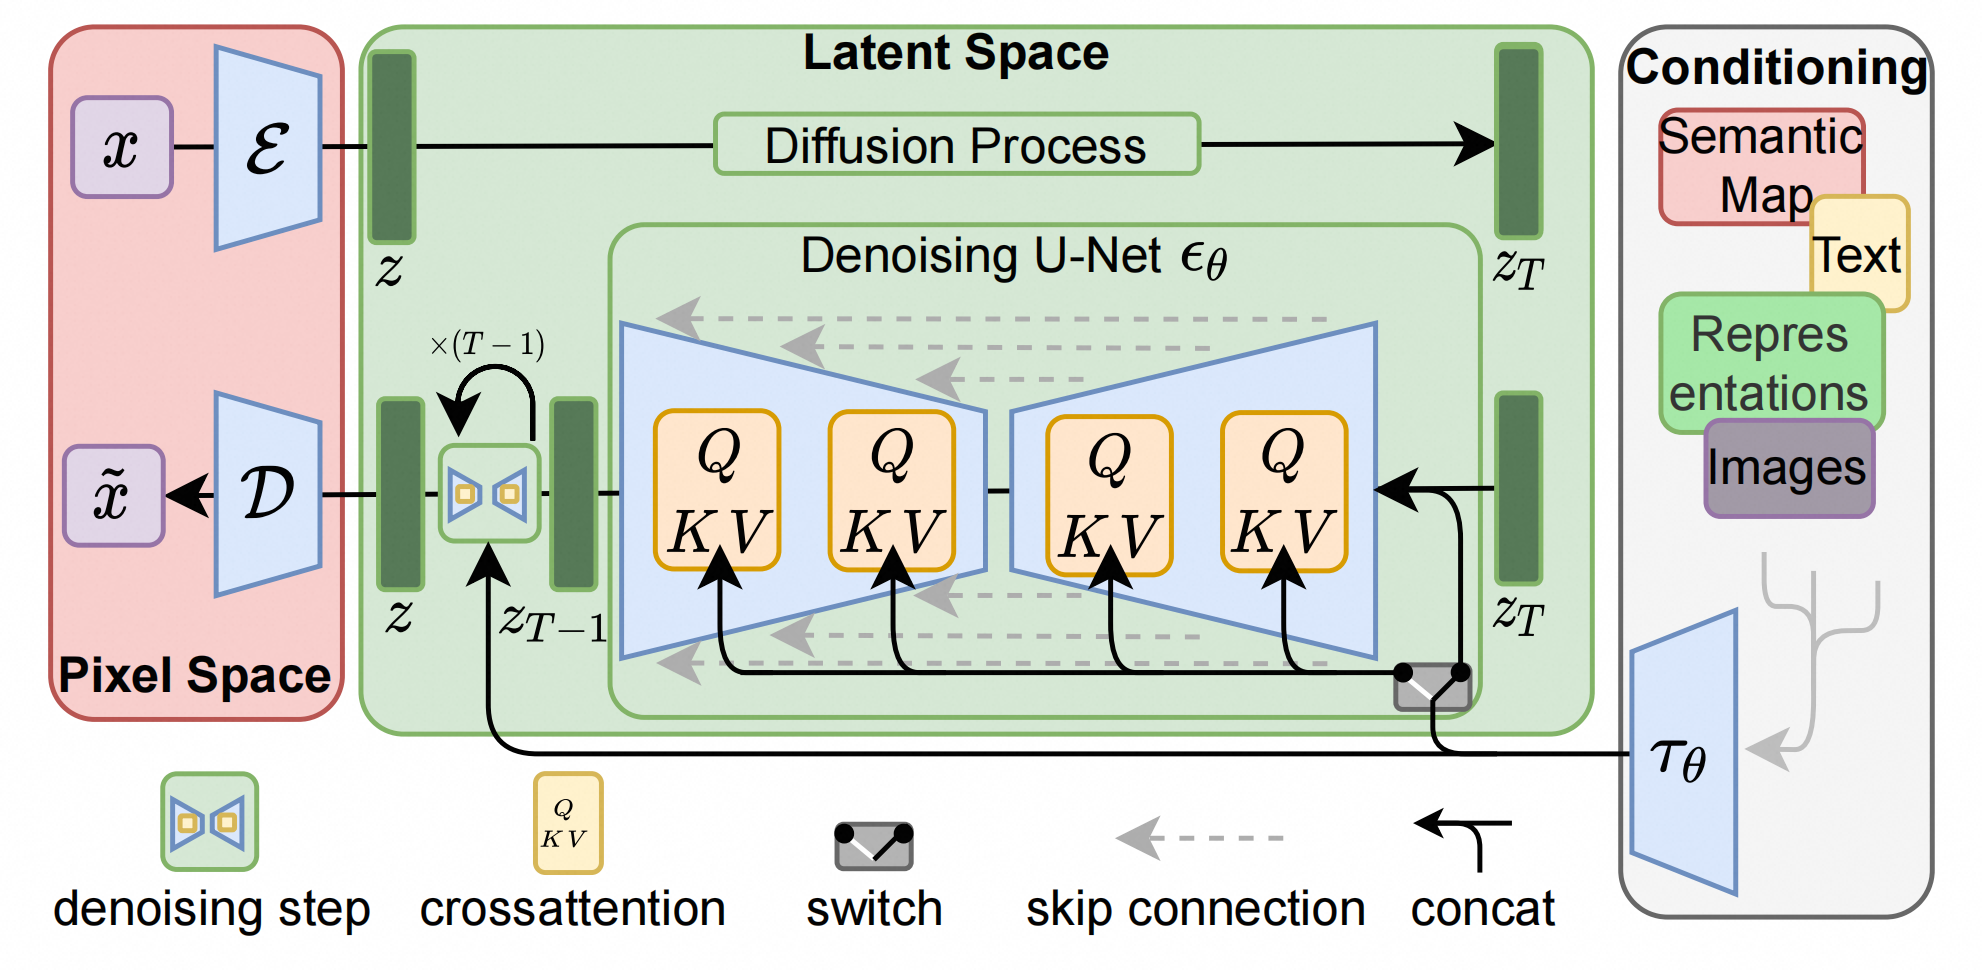
\includegraphics[width=.8\linewidth]{stable_diffusion.png}
    \caption{\label{fig:stable_diffusion}stable diffusion 架构图}
\end{figure}
\par
扩散模型中的U-Net模型主要依据注意力(attention)机制来表征数据内部(如图像的像素间)
以及数据之间(如提示文本与图像间)的关联一致性\cite{Ronneberger2015UNetCN, Radford2021LearningTV, Kruger2023TheAB},主要的模块有:
\begin{itemize}
    \item {\bfseries Self-Attention自注意力模块:}自注意力机制通过计算得到数据内部各位置之间的
    相关性和空间结构特征,帮助模型理解图像的上下文信息。它使用Q、K、V三个矩阵分别表示查询(Query)、
    键(Key)和值(Value),通过样本数据的Query与其他数据Key的点乘得到权重矩阵,进行softmax归一化
    后与Value矩阵相乘,得到最终的相关性结果\cite{Kruger2023TheAB, Liu2024TowardsUC}。
    其公式为:  
    \begin{equation}
        \text{Attention}(Q, K, V) = \text{Softmax}\left(\frac{QK^T}{\sqrt{d_k}}\right)V
    \end{equation}
    \item {\bfseries Cross-Attention交叉注意力模块:}交叉注意力机制与自注意力机制计算过程类似,与
    自注意力机制不同的是,它计算的是不同数据之间的相关性,
    比如通过将文本编码器输出的语义向量与图像特征进行相关性计算,从而引导图像生成过程与文本描述保持一致。
    具体来说,文本编码后的语义向量作为 K 和 V,图像特征作为 Q,通过图像与文本向量间的点乘来计算相关性
    \cite{Saharia2022PhotorealisticTD, Liu2024TowardsUC},
    其公式为:
    \begin{equation}
        \text{Cross-Attention}(Q_{\text{image}}, K_{\text{text}}, V_{\text{text}}) = \text{Softmax}\left(\frac{QK^T}{\sqrt{d_k}}\right)V
    \end{equation}
\end{itemize}
\par
在U-Net模型中,使用了大量的Self-Attention模块以及Cross-Attention模块来表示整个模型空间上的特征关联性,
如\autoref{fig:U-net}所示,在U-net的预测过程中,除去必要的归一化、残差层等,Self-Attention模块和Cross-Attention模块
为主要部分。
\begin{figure}[ht]
    \centering
    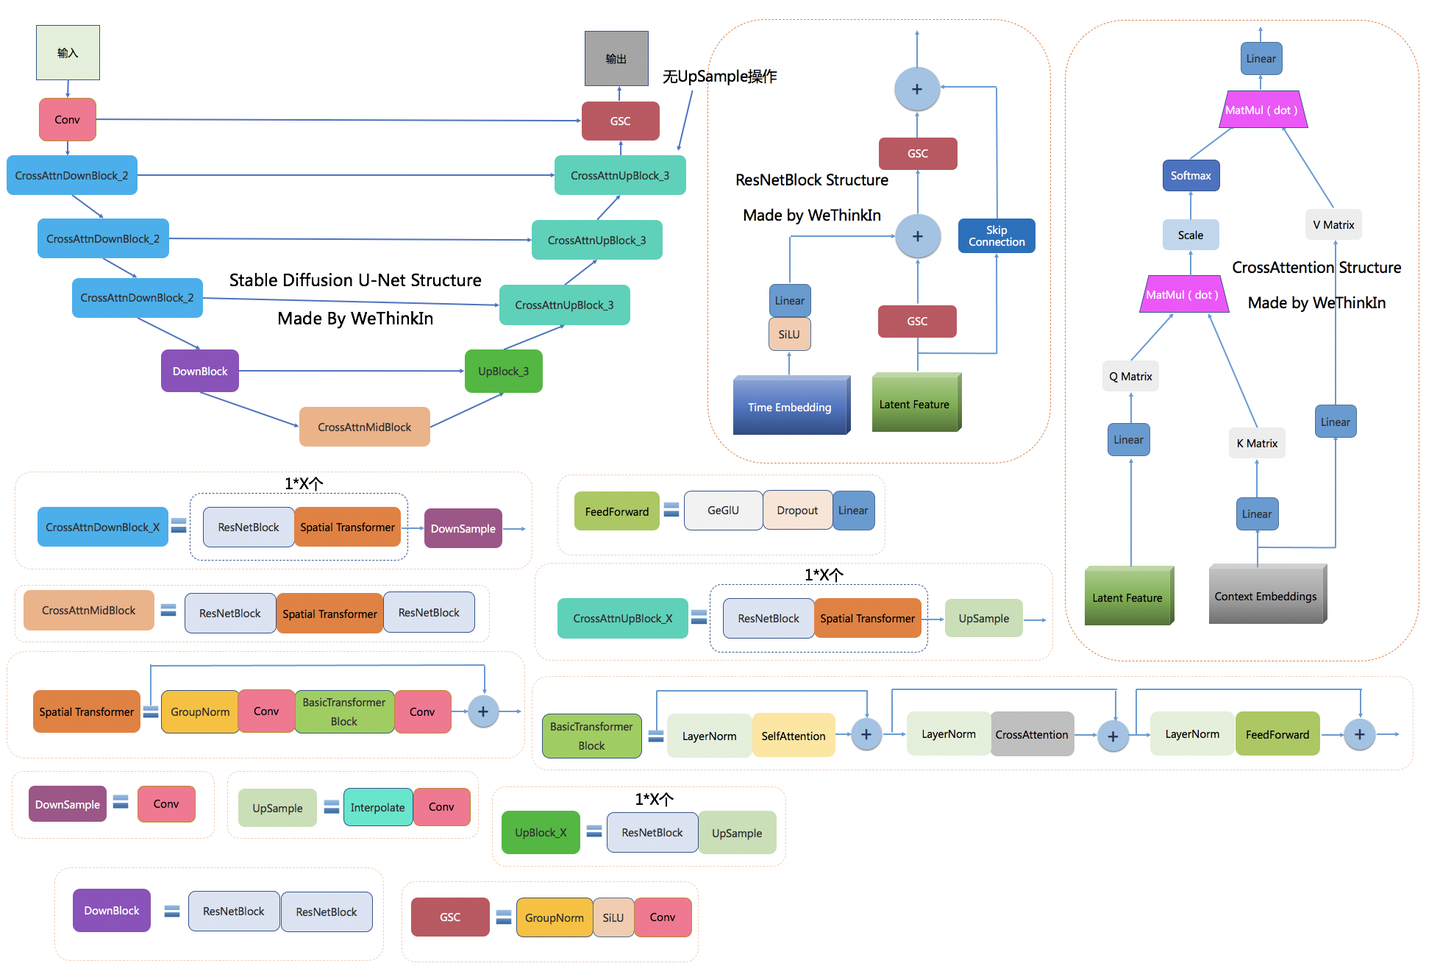
\includegraphics[width=0.85\linewidth]{U-net.png}
    \caption{\label{fig:U-net}U-net 架构图\cite{U-Net}}
\end{figure}
\subsection{扩散模型分布式推理}
\subsubsection{分布式推理的主要思想}
\par
分布式推理的核心思想是通过多GPU并行计算充分利用硬件资源,
加速模型的推理过程\cite{Shoeybi2019MegatronLMTM}。其主要策略分为{\bfseries 张量并行}(tensor 并行)和
{\bfseries 数据并行}两种方式\cite{Megatron-LM}。
\par
在张量并行中,针对大模型参数规模庞大的特点,将模型的权重按照特定维度切分,
并将不同部分部署到不同的GPU上,在扩散模型的张量并行策略中\cite{Megatron-LM},
注意力机制中的Q、K、V矩阵可以被拆分到多个GPU并行处理,最终通过通信操作(如All-Gather、broadcast等)
合并结果。
\par
在数据并行中,输入的整体数据会被划分为多个部分数据块,将每个数据块分配给不同的GPU进行并行处理。
在扩散模型的数据并行策略中,可以将输入图像分割为多个区域,
各GPU分别处理对应区域后再汇总结果。通过并行化数据处理流程,缩短了单次推理延迟。
\subsubsection{当前分布式扩散模型推理架构}
在现有的分布式扩散模型推理架构中,AsyncDiff框架主要实现张量并行,而DistriFusion框架则专注于数据并行。

\par
AsyncDiff框架采用模型切分与流水线并行策略。其核心思想是将模型按功能模块切分为多个子模型(
可根据GPU数量进行一对一或一对多分配)\cite{Chen2024AsyncDiffPD}。初始阶段输入数据需依次通过所有GPU完成预处理,
后续步骤中,各GPU基于前序缓存数据独立计算,无需等待前序GPU结果\cite{Ma2023DeepCacheAD}。
这种异步计算模式通过流水线技术实现并行加速,具体流程如\autoref{fig:AsyncDiff}所示。
\begin{figure}[ht]
    \centering
    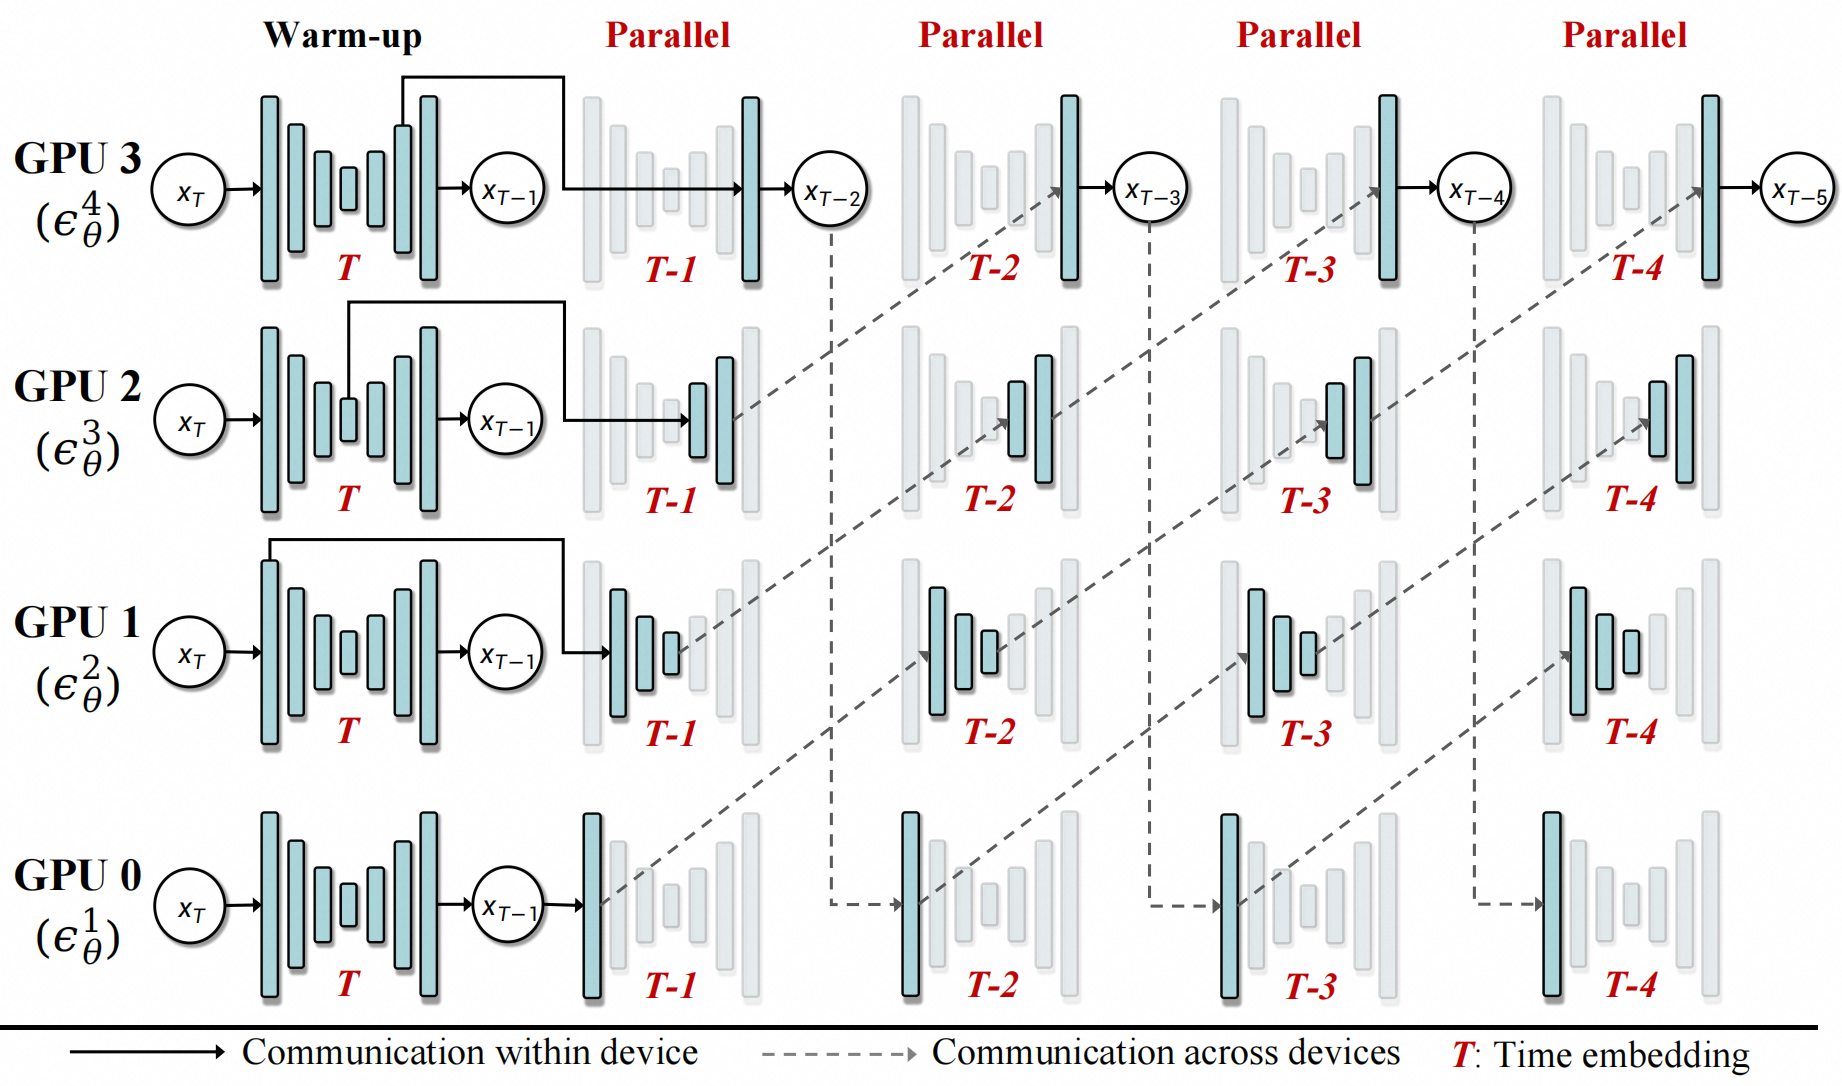
\includegraphics[width=0.8\linewidth]{AsyncDiff.png}
    \caption{AsyncDiff架构示意图\cite{Chen2024AsyncDiffPD}}\label{fig:AsyncDiff}
\end{figure}

\par
DistriFusion框架则采用数据分块并行策略。该框架为每个GPU部署完整的U-Net模型,
将输入数据划分为空间区域后分配至不同GPU进行并行预测。为保证生成图像的整体一致性,
每轮计算需通过All-Gather通信操作同步各GPU的中间输出结果以及U-Net模型参数,最终整合生成完整图像\cite{Li2024DistriFusionDP}。
其处理流程如\autoref{fig:DistriFusion}所示。
\begin{figure}[ht]
    \centering
    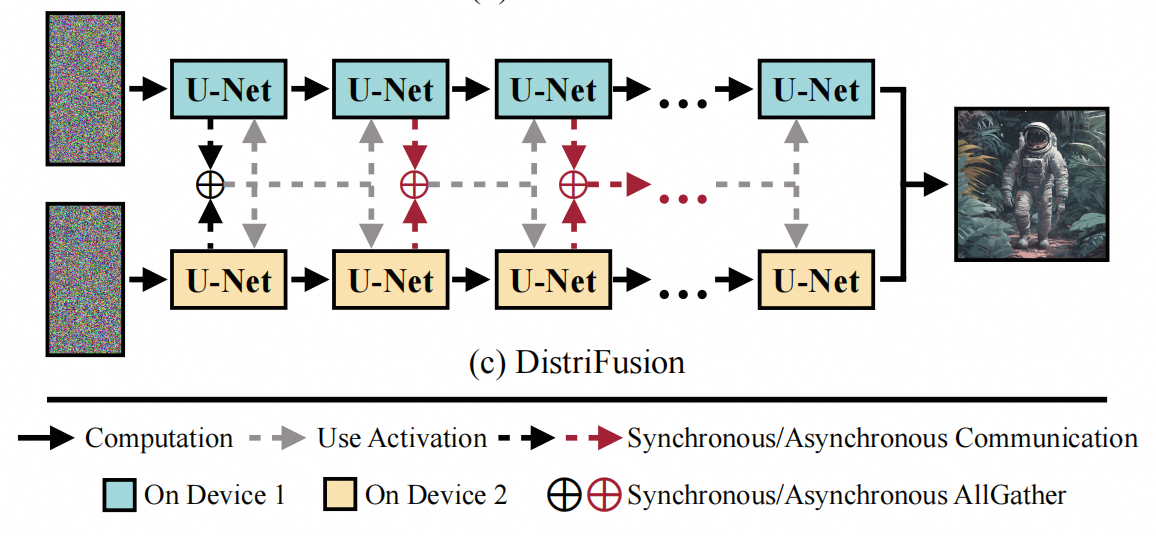
\includegraphics[width=0.6\linewidth]{Distrifusion-idea.png}
    \caption{DistriFusion架构示意图\cite{Li2024DistriFusionDP}}\label{fig:DistriFusion}
\end{figure}
\subsubsection{DistriFusion框架的推理瓶颈}
在DistriFusion框架的实际推理过程中,存在两个主要性能瓶颈:
\begin{itemize}
    \item 通信频繁:由于扩散模型具有庞大的参数量和复杂的网络结构,
    每一步迭代都需要全局同步U-Net模型参数与中间输出结果,导致通信开销显著增加;
    \item 计算需要等待通信完成:如\autoref{fig:Distrifusion-question}所示(黄色/蓝色箭头表示正常计算流程),
    在All-Gather通信操作(粉色箭头)未完成前,GPU无法启动后续计算任务。这种扩散模型去噪过程的阶段性依赖关系,
    使得计算单元需要等待通信同步完成,最终造成较大的推理延迟。
\end{itemize}
\begin{figure}[ht]
    \centering
    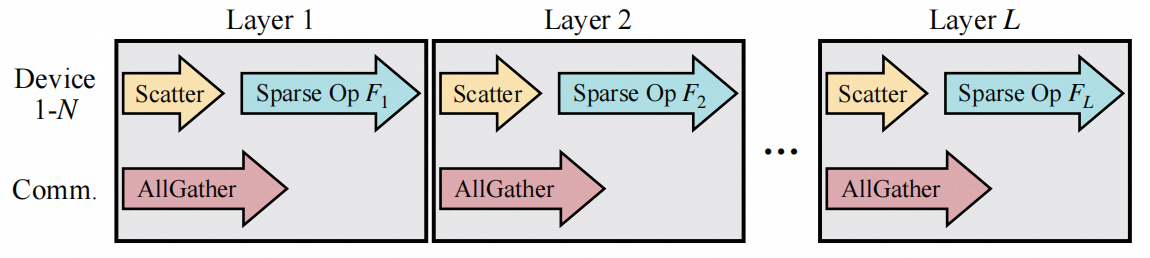
\includegraphics[width=0.8\linewidth]{Distrifusion-question.png}
    \caption{DistriFusion架构通信延迟示意图\cite{Li2024DistriFusionDP}}\label{fig:Distrifusion-question}
\end{figure}

\subsection{扩散模型分布式推理的硬件支持}
\subsubsection{GPU集群通信方式:NVLink与PCIE}
\par
在GPU集群进行分布式计算中,通信效率会直接影响整体推理性能。NVLink和PCIe是两种主流的GPU互联技术,
它们在架构设计和适用场景上存在一些差异。
\begin{itemize}
    \item NVLink是一种点对点高速互连技术,它采用GPU间直接通信,跳过CPU中转,数据传输延迟较低,带宽可达百GB/s,
    可以实现多GPU的完全互联(如8卡互联),避免出现通信瓶颈\cite{NVLink}。
    \item PCIe是一种通用性更强的传统总线标准,它使用总线共享机制,GPU间的通信通过CPU总线完成,传输数据时需要将
    数据先传回CPU总线,再将数据分发给其他GPU,相较于NVLink数据传输延迟较高\cite{PCIE}。
\end{itemize}
在选择通信方式时一般需要根据任务规模、预算和硬件条件来选择对应通信方式。NVLink性能较高,
而PCIe则以通用性和经济性适配更广泛的应用需求。
\subsubsection{高性能GPU:A100 与 RTX4090}
\par
在高性能计算领域,A100 和 RTX4090 是两款具有代表性的 GPU,在模型测试评估等方面被大量使用,
它们分别针对专业计算和消费级市场设计,具备不同的技术特点和应用场景。
\begin{itemize}
    \item A100 主要面向数据中心和科研领域,
    显存和带宽较大,能够处理复杂的深度学习模型和大规模数据集,其核心设计注重多任务协同与通信效率,
    通过 NVLink 技术实现多卡互联,大幅提高性能\cite{A100}。但在专注性能的同时,价格也较为昂贵,商用场景使用相对较少。
    \item RTX4090 则专注于消费级市场,相比与A100,RTX4090 
    在显存容量和带宽上,在单卡部署和实时渲染任务中性价比较高,商用场景使用较多\cite{RTX4090}。
\end{itemize}
两种GPU的具体参数如\autoref{tab:GPU}所示。
\begin{table}[ht]
    \centering
    \begin{tabularx}{\linewidth}{
        |>{\centering\arraybackslash}p{3cm} % 左侧固定宽度列
        |>{\centering\arraybackslash}X % 自动扩展列
        |>{\centering\arraybackslash}X| % 自动扩展列
    }
        \hline
        \textbf{指标} & \textbf{A100} & \textbf{RTX 4090} \\ \hline
        价格 & \$15,000 & \$1,600 \\ \hline
        GPU通信方式 & NVLink & PCIe \\ \hline
        GPU通信带宽 & 900 GB/s & 16 GB/s \\ \hline
    \end{tabularx}
    \caption{\label{tab:GPU}GPU型号与性能对比表\cite{A100, RTX4090, NVLink, PCIE}}
\end{table}
\par
由于商用 GPU(如 NVIDIA RTX 4090)通信传输带宽有限,使用这种GPU的情况下分布式扩散推理面临通信瓶颈。在低带宽环境
下,通信等待时间占比增加,硬件资源利用率下降,GPU 的空闲等待消耗会抵消多 GPU
分布式推理的优势。如果要充分发挥多 GPU 分布式推理,则需要部署使用 NVLink 技术的GPU 阵列(A100)\cite{Li2024DistriFusionDP},
其价格远大于传统的 PCIe 通信(RTX 4090),很大程度地限制
了分布式扩散推理的使用场景。
\subsubsection{pytorch框架GPU间通信方法}
\label{sec:pytorch-communication}
PyTorch框架是目前训练大模型的主流代码框架,其中提供了多种通信操作,用于多GPU间的数据通信,主要方法如下:
\begin{itemize}
    \item All-Reduce:将所有GPU上的整体数据进行计算聚合(如sum加法),然后将结果广播到所有GPU上,传输内容较多,通信延迟较大,
    在分布式推理中一般用于训练的预处理阶段,传递完整的参数及数据\cite{torch.distributed},如\autoref{fig:All-Reduce}所示。
    \begin{figure}[ht]
        \centering
        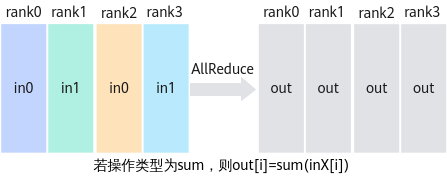
\includegraphics[width=0.6\linewidth]{All-Reduce.png}
        \caption{All-Reduce通信机制示意图\cite{All-Reduce-system}}\label{fig:All-Reduce}
    \end{figure}
    \item Broadcast:将指定GPU的数据广播到其他所有GPU上,传输内容较少,通信延迟较小\cite{torch.distributed}
    。如\autoref{fig:broadcast}所示。
    \begin{figure}[ht]
        \centering
        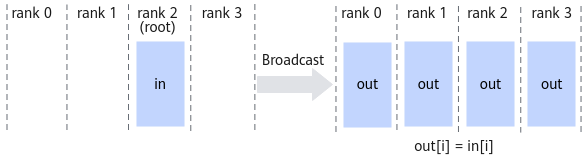
\includegraphics[width=0.8\linewidth]{broadcast.png}
        \caption{broadcast通信机制示意图\cite{All-Reduce-system}}\label{fig:broadcast}
    \end{figure}
    \item All-Gather:将所有GPU上的局部数据合并为完整数据,将结果广播到所有GPU上,
    在一些扩散模型分布式推理框架中用于后续步骤的参数及数据同步\cite{torch.distributed},如\autoref{fig:All-Gather}所示。
    \begin{figure}[ht]
        \centering
        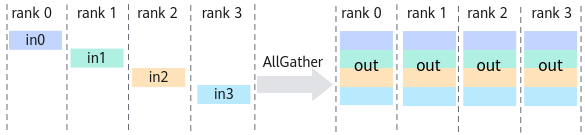
\includegraphics[width=0.8\linewidth]{All-Gather.png}
        \caption{All-Gather通信机制示意图\cite{All-Reduce-system}}\label{fig:All-Gather}
    \end{figure}
\end{itemize}
在分布式训练中时灵活运用各种通信方法,可以有效减少通信数据量,降低通信延迟,从而提高整体推理性能。

\subsection{量化指标简介}
\subsubsection{张量相似性指标}
\label{sec:tensor-similarity-metric}
\par
本文使用到三种经典的张量相似性度量方法:
\begin{itemize}
    \item \textbf{L1距离}:计算张量元素绝对差之和,反映数值层面的线性差异\cite{Distance}:
    \begin{equation}
        D_{\text{L1}}(\mathbf{x},\mathbf{y}) = \sum_{i=1}^{n} |x_i - y_i|, 
        D_{\text{L1}} \in [0,+\infty)
    \end{equation}
    \item \textbf{L2距离}:通过欧氏空间距离度量张量差异,对较大偏差更敏感\cite{Distance}:
    \begin{equation}
        D_{\text{L2}}(\mathbf{x},\mathbf{y}) = \sqrt{\sum_{i=1}^{n} (x_i - y_i)^2},
        D_{\text{L2}} \in [0,+\infty)
    \end{equation}
    \item \textbf{余弦相似度}:衡量张量向量空间中的方向一致性,忽略幅值差异\cite{CosineSimilarity}:
    \begin{equation}
        S_{\cos}(\mathbf{x},\mathbf{y}) = \frac{\mathbf{x} \cdot \mathbf{y}}{\|\mathbf{x}\| \|\mathbf{y}\|},
        S_{\cos} \in [-1,1]
    \end{equation}
\end{itemize}
\par
L1/L2距离适用于数值敏感场景,余弦相似度则擅长捕捉结构相似性。

\subsubsection{图像质量指标}
\label{sec:image-quality-metric}
\par
本文采用三种图像质量评估指标来对图像质量进行全面评估:
\begin{itemize}
    \item \textbf{PSNR(峰值信噪比)}:衡量像素级精度,值域使用对数尺度\cite{ceshizhibiao}:
    \begin{equation}
        \text{PSNR} = 10 \cdot \log_{10}\left(\frac{\text{MAX}^2}{\text{MSE}}\right)
    \end{equation}
    其中$\text{MAX}$为像素最大值(如255),$\text{MSE}$为均方误差\cite{Wang2019SpatialAS}。
    
    \item \textbf{FID(Fréchet起始距离)}:评估生成图像与真实图像的分布相似性\cite{ceshizhibiao}:
    \begin{equation}
        \text{FID} = \|\mu_r - \mu_g\|^2 + \text{Tr}(\Sigma_r + \Sigma_g - 2\sqrt{\Sigma_r\Sigma_g})
    \end{equation}
    其中$(\mu_r, \Sigma_r)$和$(\mu_g, \Sigma_g)$分别表示真实与生成图像在Inception-v3特征空间的统计量
    \cite{Heusel2017GANsTB}。
    
    \item \textbf{LPIPS(学习感知相似度)}:基于深度特征距离的感知相似性度量\cite{ceshizhibiao}:
    \begin{equation}
        \text{LPIPS} = \sum_{l} \frac{1}{H_lW_l} \sum_{h,w} \|w_l \odot (\phi_l(I_1)_{hw} - \phi_l(I_2)_{hw})\|_1
    \end{equation}
    其中$\phi_l$表示预训练VGG网络的第$l$层特征,$w_l$为可学习权重\cite{Zhang2018TheUE}。
\end{itemize}
\par
其中,PSNR更关注像素精度,FID主要用来评估分布匹配度,LPIPS侧重于人类视觉感知特性,
三者形成全面质量评估体系。 

\section{基础研究工作}
本章从扩散模型(使用stable diffusion模型)的推理特性出发,以 Distrifusion 框架为基准,
系统分析其分布式推理过程中的模块通信机制。同时通过相邻步骤间的相似性特征,提出通信优化的理论依据与实践启发。
\subsection{扩散模型推理特点}
\subsubsection{扩散模型推理过程}
\label{sec:diffusion_model_inference_process}
Stable Diffusion 模型推理过程为U-Net模型,其中包括自注意力层(Self-Attention)、交叉注意力层(Cross-Attention)
和残差网络块(ResNet Block)\cite{rombach2022high, Ronneberger2015UNetCN}等。为后续深入分析分布式推理时的通信特性,需要明确以下信息:
\begin{itemize}
    \item 模块激活过程:推理过程中实际被调用的模块以及激活顺序;
    \item 模块数量统计:各类型模块的数量分布(为后续分布式推理时的通信量分析提供参考);
    \item 模块依赖关系:模块间的输入输出连接状态。
\end{itemize}
\par
基于上面的需求,通过算法 \ref{alg:tracking} 对SDXL\cite{Podell2023SDXLIL}的U-Net模型进行量化分析,遍历模型所有层,
记录每种模块(如 Self-Attention、ResNet Block 等)的数量,为每个非叶节点模块分配唯一ID,
并基于模块的输入张量追踪其依赖关系,最终生成模块依赖图。
\begin{algorithm}[!h]
    \caption{扩散模型推理跟踪记录}
    \label{alg:tracking}
    \renewcommand{\algorithmicrequire}{\textbf{Input:}}
    \renewcommand{\algorithmicensure}{\textbf{Output:}}
    \begin{algorithmic}[1]
        \REQUIRE Model $M$
        \ENSURE Module counter $C$, Graph $G = (V, E)$
        \STATE Initialize $C \leftarrow \{\}$, $E \leftarrow \{\}$, $id \leftarrow 0$
        \FOR{layer $\in \mathcal{M}$.modules()}
            \IF{layer is non-leaf}
                \STATE $t \leftarrow$ type of layer
                \STATE $C[t] \leftarrow C[t] + 1$ \COMMENT{Update counter}
                \STATE assign $id$ to layer
                \FOR{input $\in$ layer.inputs}
                    \STATE add edge $(input.id, id)$ to $E$
                \ENDFOR
            \ENDIF
        \ENDFOR
        \RETURN $C, G$
    \end{algorithmic}
\end{algorithm}
测试结束后统计各模块实例数量并构建模块间依赖图,为后续分布式推理的通信分析提供参考,如\autoref{fig:module-graph}所示,
U-Net模型内的模块主要包括:
\begin{itemize}
    \item \textbf{编码器}(DownBlock 与 CrossAttnDownBlock):  
    通过多级下采样逐步提取特征;
    每级分别包含残差块(ResNet Block)与注意力层(Self-Attention与Cross-Attention)。
    \item \textbf{中间块}(MidBlock):处理编码器输出的高层特征,强化全局语义。
    \item \textbf{解码器}(UpBlock 与 CrossAttnUpBlock):  
    通过上采样恢复特征,结合跳跃连接(Skip Connection)传递编码器低层特征,保留一些细节信息\cite{Ronneberger2015UNetCN}。
\end{itemize}
模型主要包含主要包含70个 Self-Attention层、
70个 Cross-Attention层、17个 ResNet Block层。可以看到,注意力层占比较多(共 140 层),
在推理过程中占据核心计算资源,后续需要重点关注其通信开销。
\begin{figure}[ht]
    \centering
    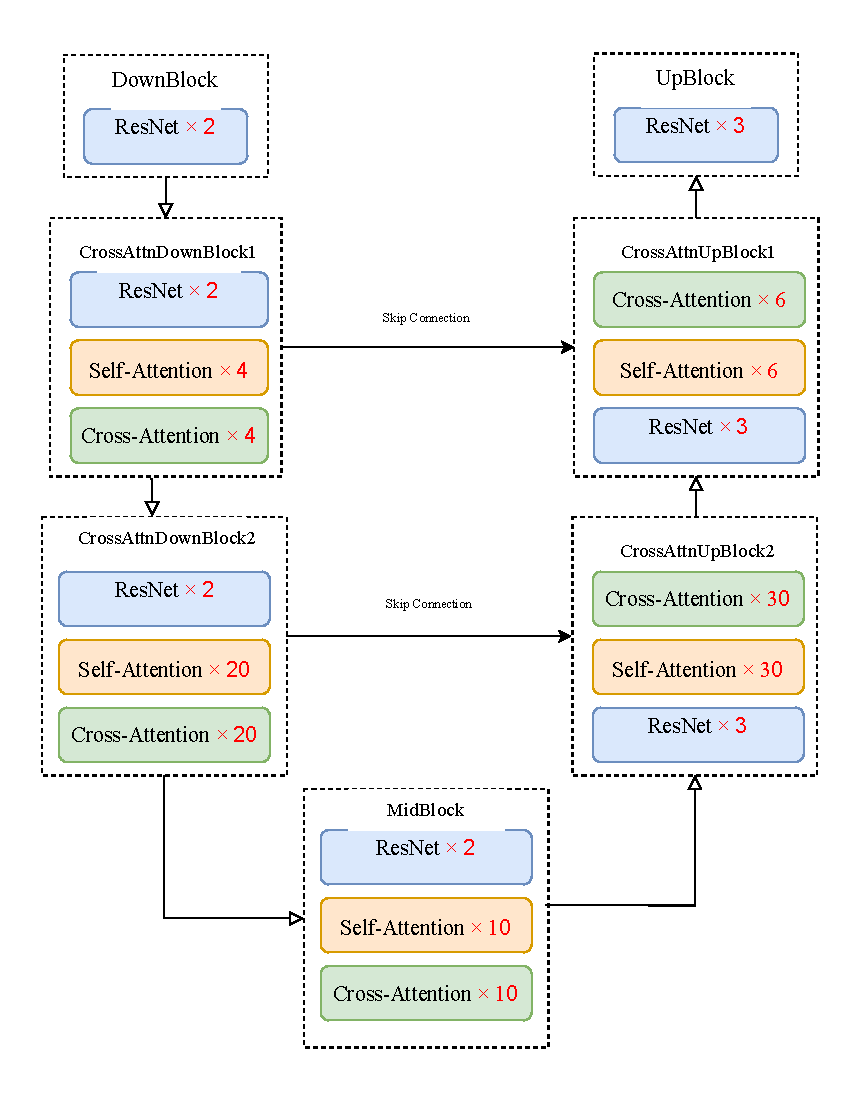
\includegraphics[width=0.6\linewidth]{module-graph.pdf}
    \caption{U-Net模型具体模块架构图}\label{fig:module-graph}
\end{figure}
\subsubsection{扩散模型分布式推理各模块通信参数量及储存空间}
\label{sec:diffusion_model_distributed_inference_communication_parameter}
\par
在基于 Distrifusion 的扩散模型分布式推理框架中,推理阶段通过将输入数据划分为多个数据分
片并分配至不同 GPU 进行并行处理。为确保各数据分片的计算一致性,需要在每轮推理前引入 GPU 间通信机制。
为量化分析具体通信开销\cite{Li2024DistriFusionDP},本节测试了 U-Net 模型中各模块在推理阶段具体传输的参数量,
明确了通信优化时需要重点考虑及处理的模块,
从而为后续通信优化策略(如通信-计算重叠)提供数据支撑。
\par
根据\ref{sec:diffusion_model_inference_process}节对Distrifusion框架推理过程的分析,在推理过程中的核心模型U-Net主要包含 Self-Attention 层、
Cross-Attention 层和 ResNet Block 层,因此,在分布式推理过程中,
需要测试这三个模块具体的通信同步情况,如是否进行通信同步、通信总量等等。
根据需要使用简单的getBytes()函数获取张量在通信过程中传输的的数据量,在双卡GPU下进行测试,对每个模块的
通信过程进行遍历,如算法 \ref{alg:simple_comm}所示。
\begin{algorithm}[!h]
    \caption{各模块参数量统计}
    \label{alg:simple_comm}
    \renewcommand{\algorithmicrequire}{\textbf{Input:}}
    \renewcommand{\algorithmicensure}{\textbf{Output:}}
    \begin{algorithmic}[1]
        \REQUIRE Model $M$
        \ENSURE Total communication volume $V$
        \STATE Initialize $V \leftarrow 0$
        \FOR{layer $\in$ $M$.modules()}
            \IF{layer is non-leaf}
                \FOR{input $\in$ layer.inputs}
                    \STATE $V \leftarrow V + \text{nccl.getBytes}(input.tensor)$
                \ENDFOR
                \FOR{output $\in$ layer.outputs}
                    \STATE $V \leftarrow V + \text{nccl.getBytes}(output.tensor)$
                \ENDFOR
            \ENDIF
        \ENDFOR
        \RETURN $V$
    \end{algorithmic}
\end{algorithm}
测试统计结果(如图 \ref{fig:module-param} 所示)表明,各模块在通信量分布上呈现显著差异:
\begin{itemize}
    \item 在总体通信开销中Self-Attention 层占比较大,其通信量占比超过 90\%,尤其在 3072×3072等高分辨率场景下,
    通信量接近 1000 MB,是导致通信延迟的主要部分。
    \item Cross-Attention 无通信开销:由于其设计特性,不产生跨设备通信需求\cite{Zhang2024FasterDV}。
    \item ResNet Block 通信量占比不足 10\%,通信需求较低。
\end{itemize}
\begin{figure}[ht]
    \centering
    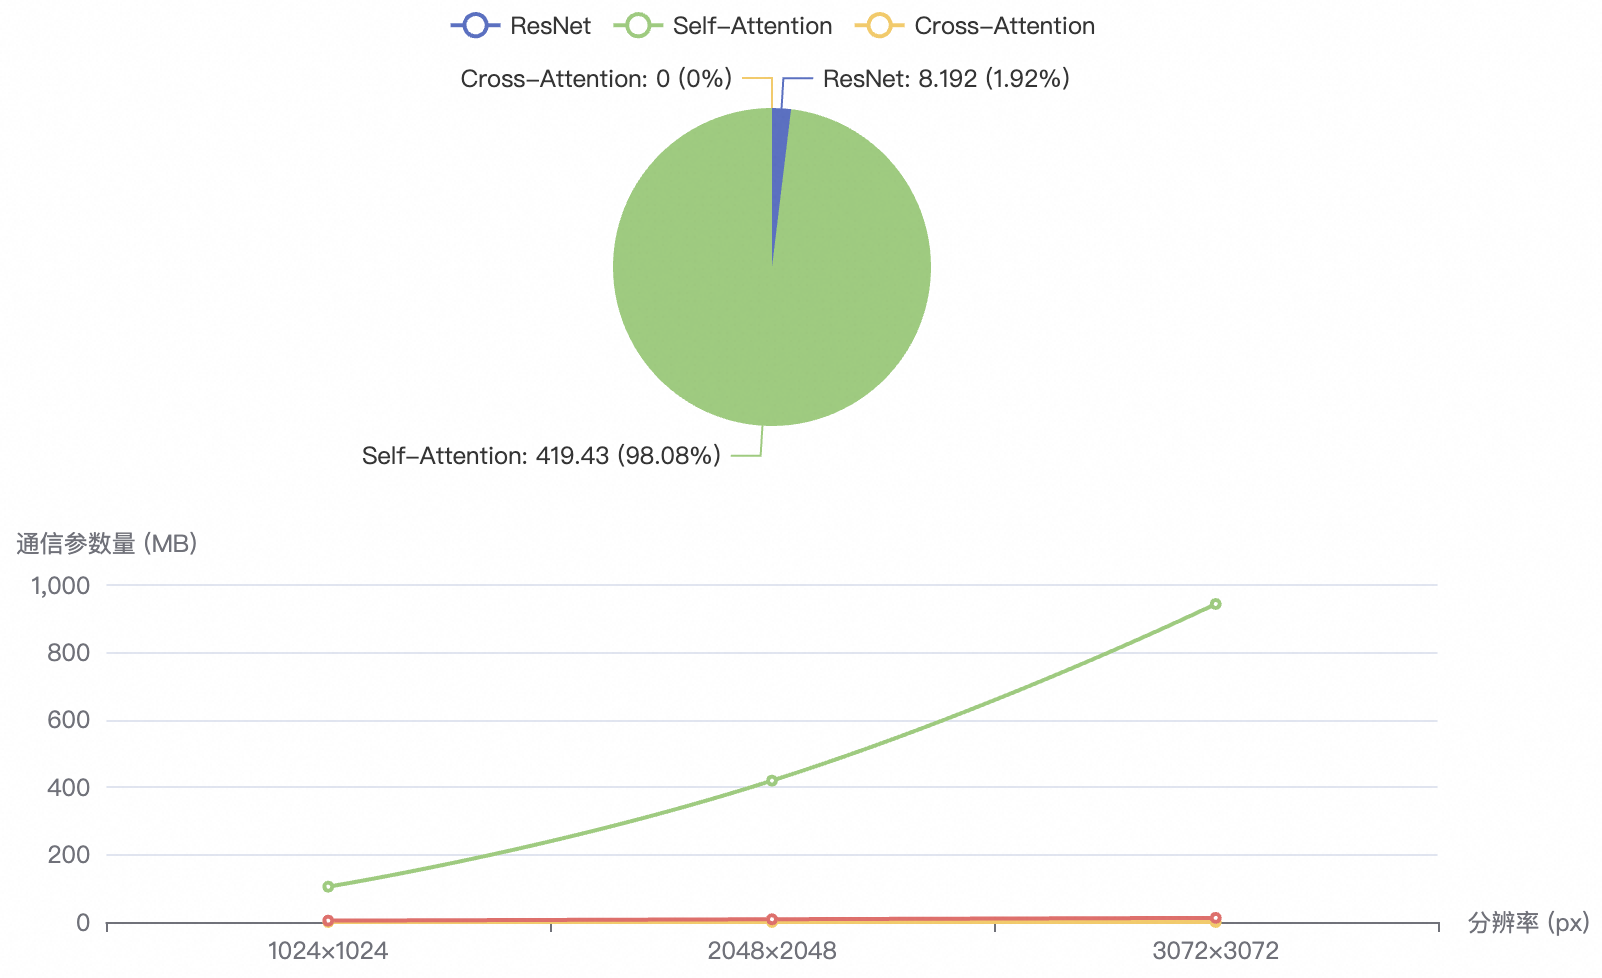
\includegraphics[width=0.9\linewidth]{module-param.png}
    \caption{各模块分布式推理时通信量}\label{fig:module-param}
\end{figure}
\par
同时,在分布式推理场景中,随着 GPU 数量的增加,通信开销呈现线性增长趋势(如图 \ref{fig:GPU-communication} 所示)。
以双卡环境为例,每个 GPU 的本地数据量为 $ t/2 $,需与对端 GPU 传输 $ t/2 $ 数据,
总通信量为 $ t $(即 $ t/2 \times 2 $)。然而,当扩展至 4 卡系统时,
尽管单卡数据量降至 $ t/4 $,每个 GPU 需与其他 3 个 GPU 通信,导致总通信量升至 $ 3t $($ 3t/4 \times 4 $);
进一步扩展至 8 卡系统时,总通信量达到 $ 7t $($ 7t/8 \times 8 $),是双卡系统的 7 倍。
这一趋势可一般化为 $ (N-1)t $,其中 $ N $ 为 GPU 数量,通信开销与 GPU 数量呈线性增长关系。
虽然单卡传输量随 $ N $ 增大而降低($ t/N $),但通信路径数按 $ O(N^2) $ 级别增长,在计算量减小的情况下,
进一步暴露通信延迟。
\begin{figure}[ht]
    \centering
    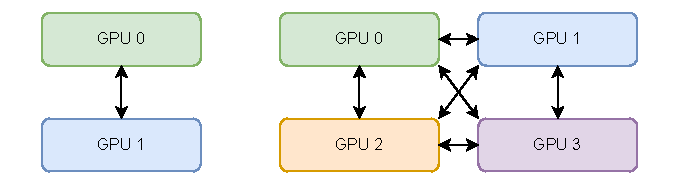
\includegraphics[width=0.8\linewidth]{GPU-communication.pdf}
    \caption{不同 GPU 数量下通信数据流向。}
    \label{fig:GPU-communication}
\end{figure}
\par
除了通信延迟外,扩散模型在推理过程中对显存资源的占用也较高。尤其在进行分布式推理时,由于大量使用缓存机制,
显存不足的问题尤为常见\cite{Ma2023DeepCacheAD}。为此,本文基于 Distrifusion 框架测试了在1024×1024分辨率下推理过程中的显存使用
情况,重点关注通信占比较高的 Self-Attention 层中的 Q、K、V 矩阵。如图 \ref{fig:GPU-memory} 所示,
整个推理过程中各Self-Attention 层所需的缓存空间较大,对硬件资源提出了很高要求。
\begin{figure}[ht]
    \centering
    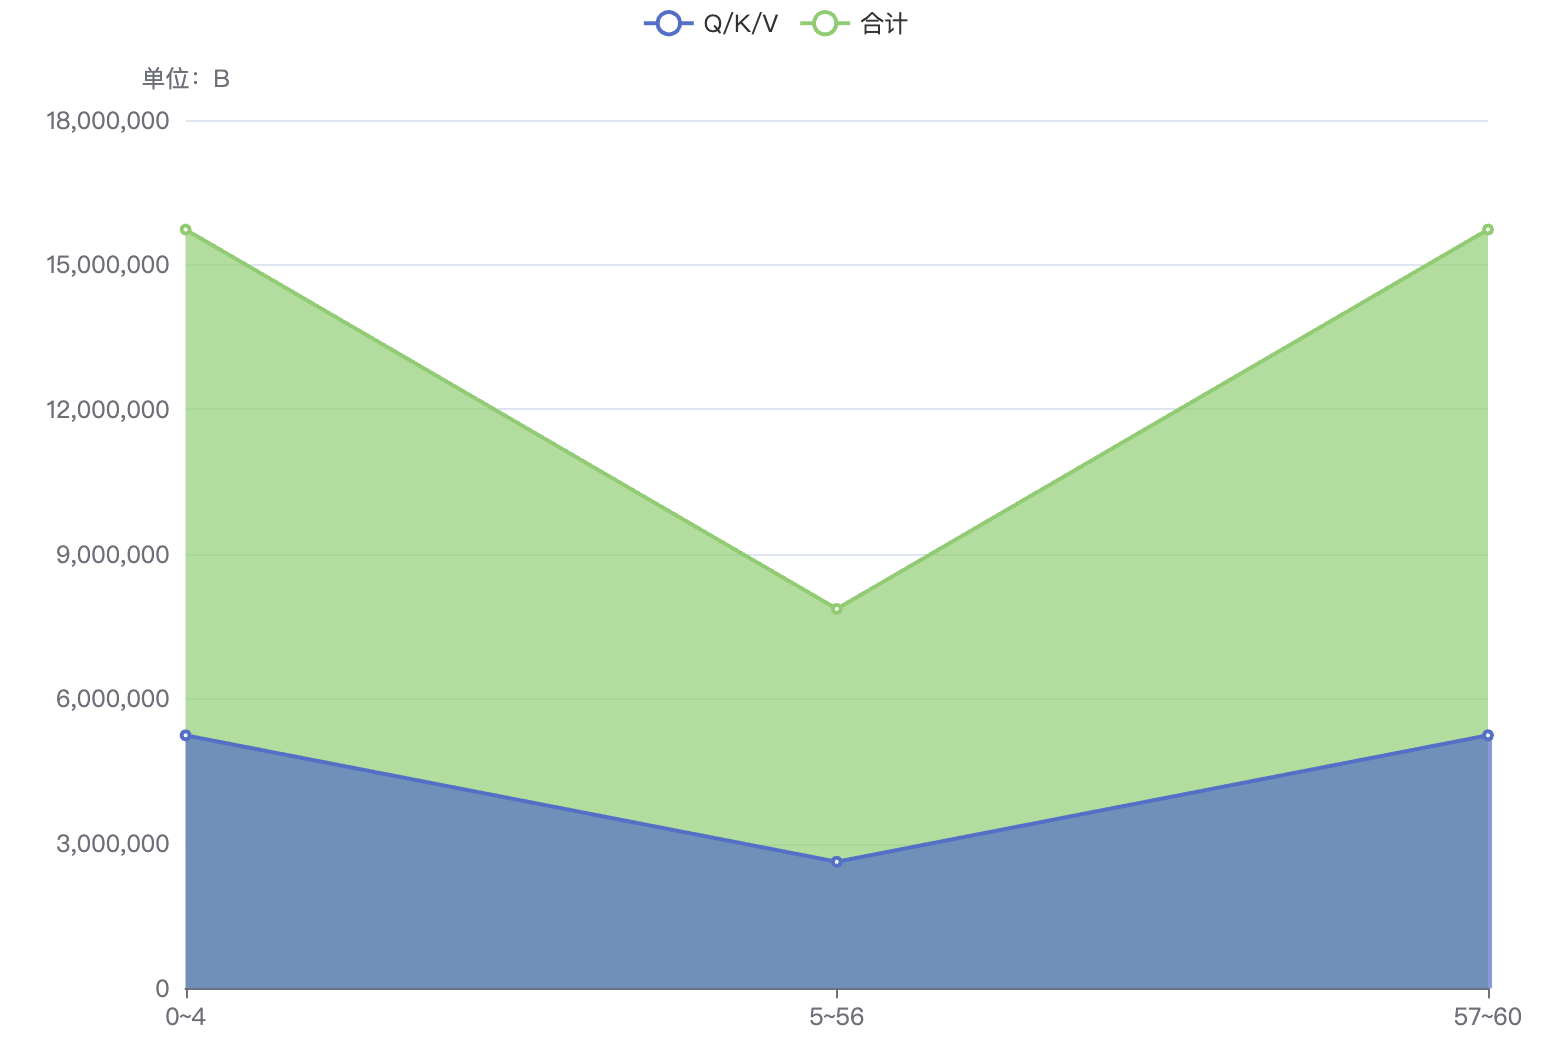
\includegraphics[width=0.7\linewidth]{GPU-memory.png}
    \caption{Distrifusion在1024×1024 分辨率下推理时各Self-Attention 层 Q、K、V 矩阵的缓存空间大小}
    \label{fig:GPU-memory}
\end{figure}
\par
通过总结可以得到,在Distrifusion框架分布式推理过程中,Self-Attention 层通信量占据绝大部分,是通信延迟的主要来源。
随着输入图像分辨率以及GPU数量的提高,通信延迟占比显著增加,成为制约整体推理速度的主要瓶颈。同时,过多的通信缓存
会导致显存使用量增加,从而可能导致在一些设备上显存不足的问题。
因此,在后续的通信优化策略中,需要重点关注 Self-Attention 层的通信同步策略,从而减少通信延迟及显存使用量。

\subsubsection{扩散模型推理阶段相邻步骤相似性分析}
\label{sec:diffusion_model_inference_process_similarity}
目前的研究表明,扩散模型推理过程中相邻去噪步骤间存在显著的数据相似性\cite{Cao2022ASO},
这一特性使得步骤压缩策略与数据缓存机制有很好的效果,通过存储中间步骤特征数据可有效减少冗余计算\cite{Ma2023DeepCacheAD, Zhang2024FasterDV}。
在分布式推理场景下,可以将这个特性用于降低跨设备通信开销,但需要在生成质量与通信效率间取得平衡。
为此,本研究聚焦于扩散模型推理阶段Self-Attention层的参数相似性分析(由\label{sec:diffusion_model_distributed_inference_communication_parameter}
节证实为通信瓶颈所在部分)。
\par
在Self-Attention机制中,核心通信开销集中于K、V矩阵的GPU间通信。
实验数据统计显示(如\autoref{fig:KV-similarity}横坐标为推理步数,纵坐标为余弦相似度,不同颜色曲线表示
不同Self-Attention层),
相邻推理步骤间的K/V矩阵存在显著的相似性,
这一结果为通信优化提供了关键的理论依据,通过量化相似度可以决定缓存通信冻结和缓存复用策略,
在保证生成质量的同时实现通信优化\cite{Liu2021AutoFreezeAF}。
进一步分析图 \ref{fig:KV-similarity} 中的数据可以发现,扩散模型在推理阶段相邻步骤之间的 KV 相似性整体较高,
余弦相似度始终超过 0.984。然而,在不同的推理时间步中,各 Self-Attention 层之间的相似性仍存在一定差异。例如,
图中浅紫色曲线所代表的某 Self-Attention 层在第九步时其 K/V 矩阵的余弦相似度明显低于其他层,
显示出与其他步骤之间更高的变化性。因此,在后续算法设计中,对于此类相似性较低、变化较大的层应适当降低通信抑制,
以避免图像质量下降。
\par
除K/V矩阵相似性外,在Distrifusion分布式推理框架中,各推理步骤的输出特征图也需要跨GPU同步,
因需要进一步量化分析相邻步骤输出结果的相似性。本文采用L2范数衡量输出特征差异,实验结果如图
\ref{fig:output-similarity}所示,横轴为推理步数,纵轴为计算所得相似度值(归一化后),
不同颜色曲线对应不同Self-Attention层。
\begin{figure}[ht]
    \centering
    % 第一张图
    \begin{minipage}[t]{0.45\linewidth}
        \centering
        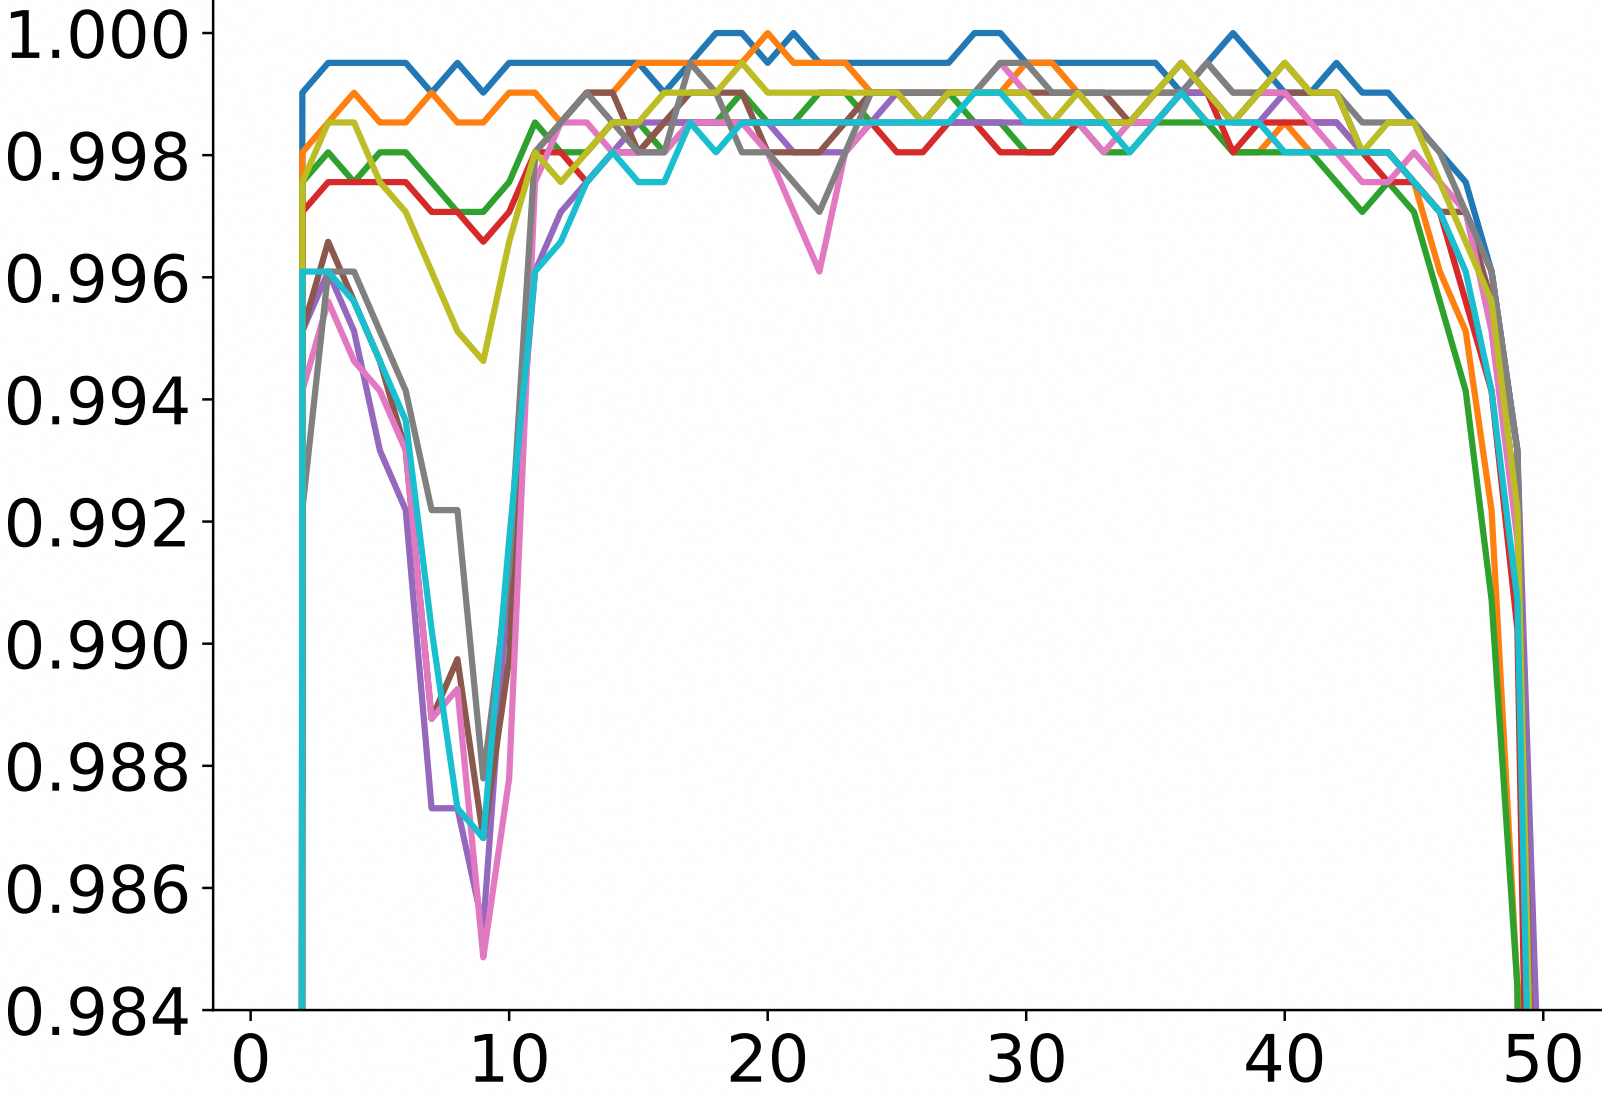
\includegraphics[width=\linewidth]{KV-similarity.png}
        \caption{扩散模型推理阶段部分Self-Attention层相邻步骤KV相似性}
        \label{fig:KV-similarity}
    \end{minipage}
    \hfill % 自动填充水平间距
    % 第二张图
    \begin{minipage}[t]{0.45\linewidth}
        \centering
        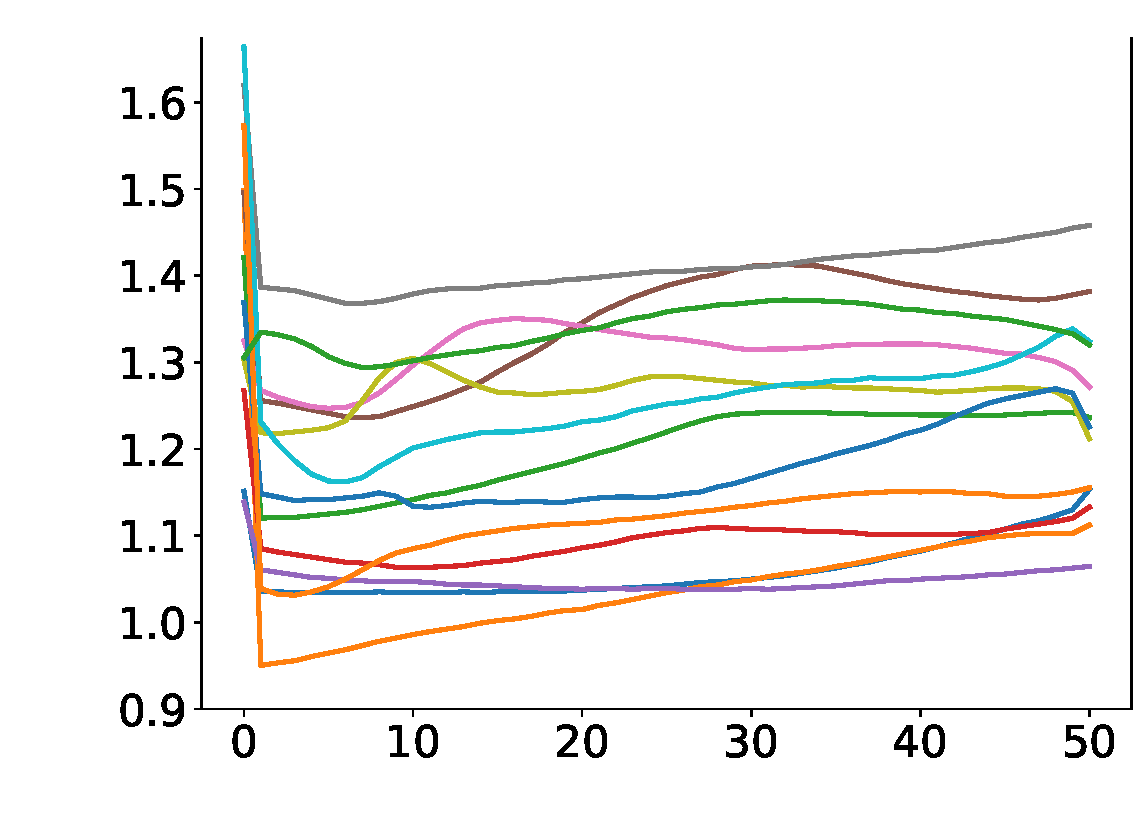
\includegraphics[width=\linewidth]{output-similarity.pdf}
        \caption{扩散模型推理阶段部分Self-Attention层相邻步骤输出结果相似性}
        \label{fig:output-similarity}
    \end{minipage}
\end{figure}
数据显示,扩散模型推理过程中相邻步骤输出特征具有显著相似性(L2距离集中于0.9-1.5区间)。
同样,不同层之间的相似性也存在差异,因此,需要细致的通信抑制算法来平衡计算效率与生成质量。
\subsection{扩散模型分布式推理框架的通信延迟}
\label{sec:diffusion_model_distributed_inference_communication_delay}
\par
在扩散模型分布式推理框架DistriFusion中,下面的实验表明通信延迟是限制其在商用GPU集群上运行速度的关键瓶颈。
为深入量化分析通信开销占比及其优化潜力,本文在多GPU集群(2/4/8卡)、多分辨率(512×512/1024×1024)以及
使用低带宽PCIe网络连接的RTX 4090GPU集群条件下,
系统性地测量了端到端推理延迟与GPU间通信耗时(详见\autoref{fig:communication-delay-1024}和
\autoref{fig:communication-delay-512})。
\begin{figure}[ht]
    \centering
    \begin{minipage}[t]{0.45\linewidth}
        \centering
        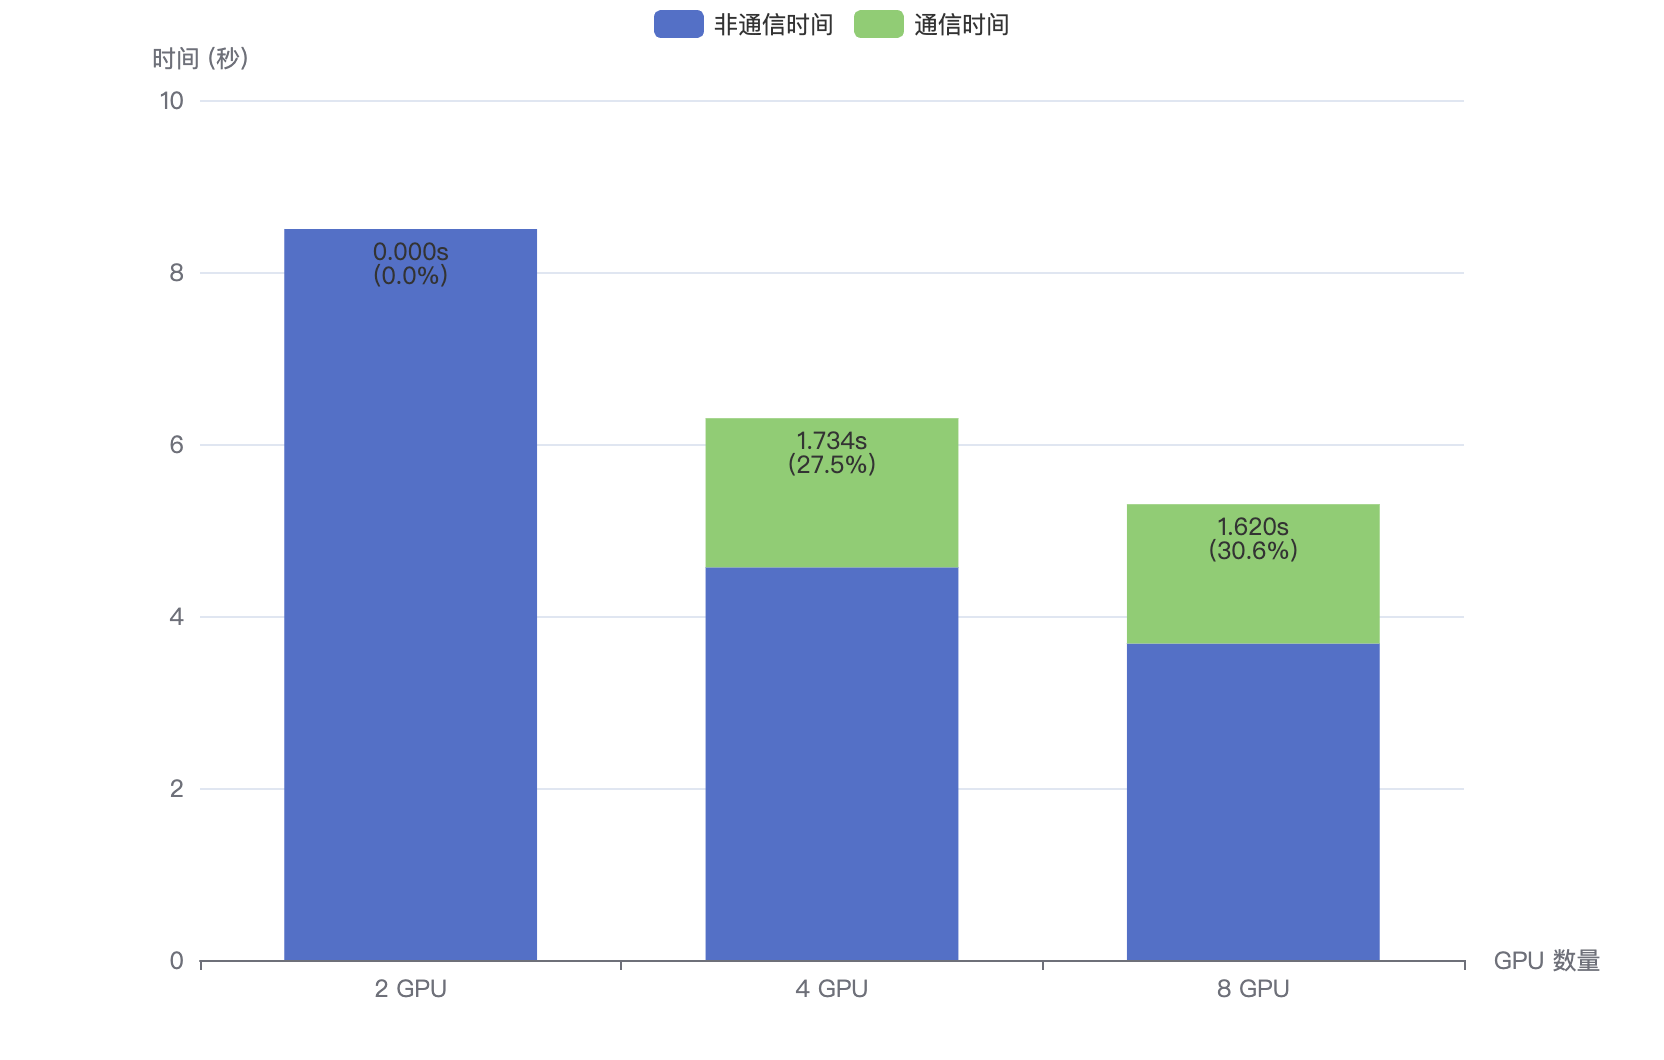
\includegraphics[width=\linewidth]{communication-delay-1024.png}
        \caption{1024×1024分辨率,不同GPU数量下GPU通信时间占比(使用搭载了PCIe网络连接的RTX 4090 GPU集群)}
        \label{fig:communication-delay-1024}
    \end{minipage}
    \hfill
    \begin{minipage}[t]{0.45\linewidth}
        \centering
        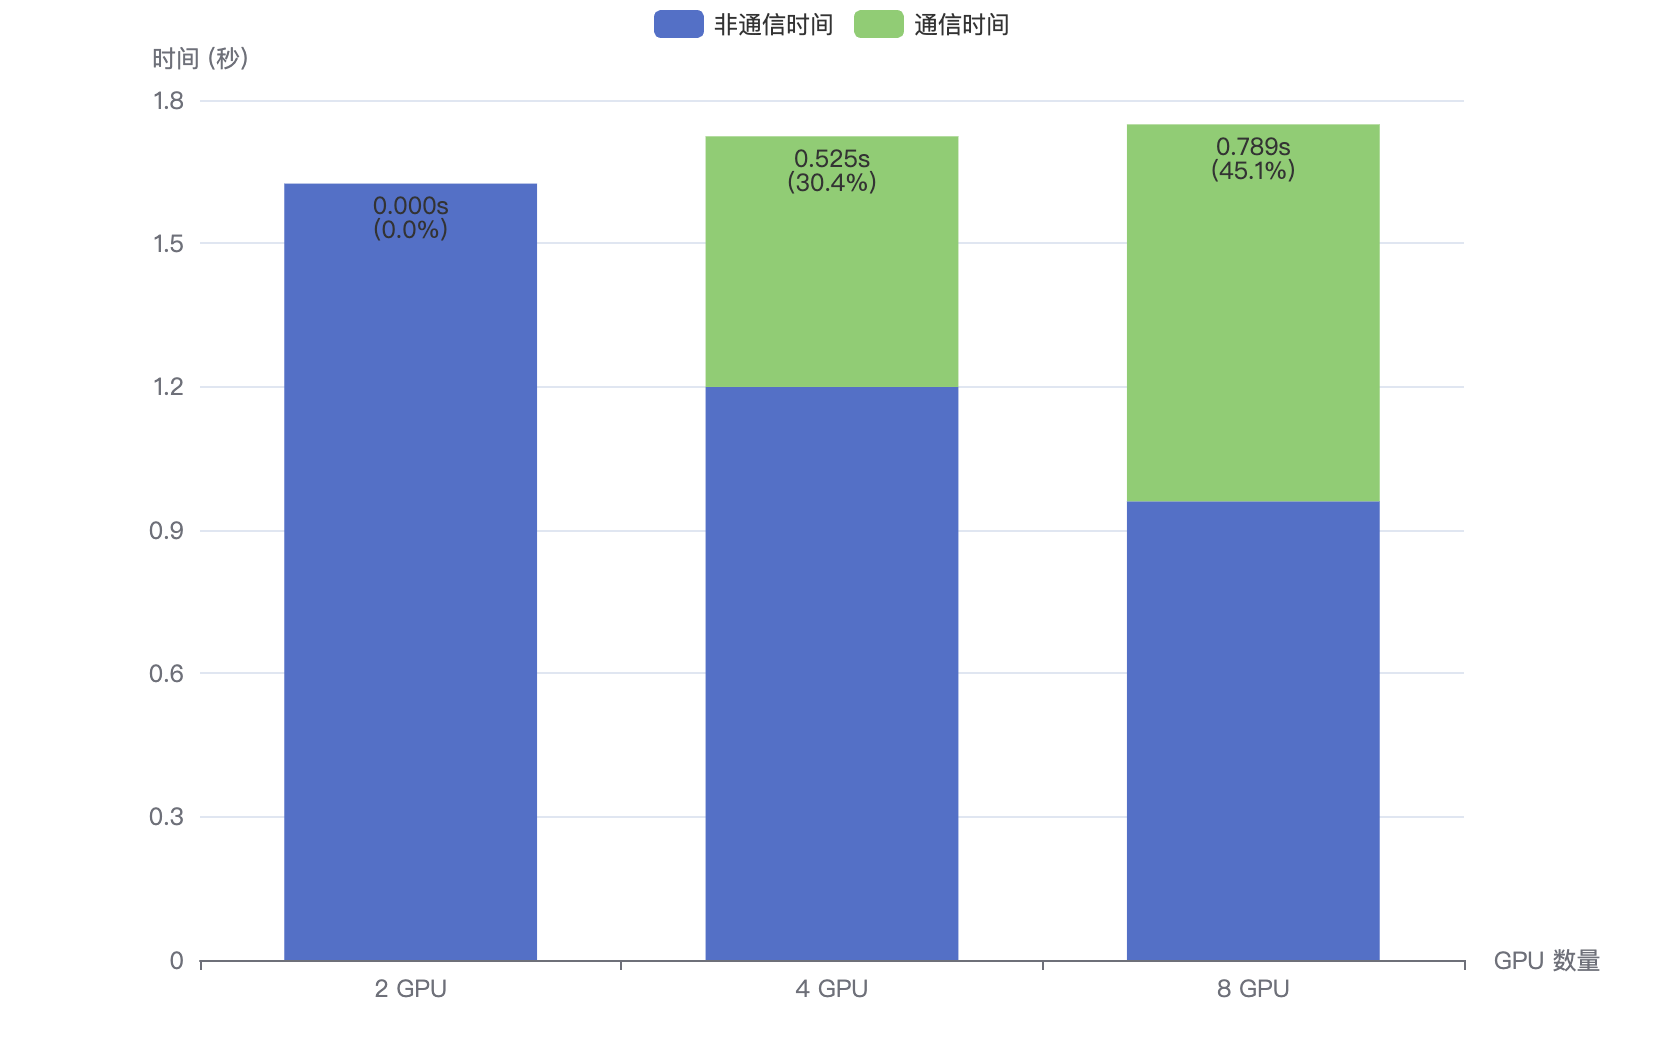
\includegraphics[width=\linewidth]{communication-delay-512.png}
        \caption{512×512分辨率,不同GPU数量下GPU通信时间占比(使用搭载了PCIe网络连接的RTX 4090 GPU集群)}
        \label{fig:communication-delay-512}
    \end{minipage}
\end{figure}
\par
实验数据显示,通信延迟在低带宽商用GPU场景下成为关键的性能瓶颈。,在512×512和1024×1024分辨率下,
4GPU与8GPU配置的通信延迟占比接近30\%-40\%,造成大量GPU资源闲置。
同时,当GPU数量增加时,通信延迟占比也进一步提高,导致多GPU并行加速收益被部分抵消。
这些发现表明,通过通信策略优化和计算-通信重叠技术来降低通信开销,可使整体推理性能有较大提升。
\par
\subsection{研究启发}
从上面的研究中可以发现,当前基于Distrifusion框架的扩散模型分布式推理在商用GPU(如RTX 4090)
低带宽场景中存在显著通信瓶颈。具体而言,该问题主要由三个因素共同作用导致:
\begin{itemize}
    \item Self-Attention层的频繁通信:Self-Attention层的K/V矩阵在分布式计算中会产生大量通信开销
    \item GPU集群扩展的通信需求:随着计算节点数量增加,跨GPU通信需求呈线性增长
    \item PCIe总线的带宽限制:商用GPU间通过PCIe互联时,带宽较低
\end{itemize}
通过量化分析不同迭代步间的参数矩阵相似度,我们发现两个关键特征:
\begin{itemize}
    \item 相邻迭代步的K/V矩阵具有高度相似性
    \item 相邻迭代步的输出结果也具有一定的相似性
\end{itemize}

基于上述发现,我们可以通过通信冻结并且优化异步传输机制为低带宽商用GPU环境下的高效分布式推理提供新的解决方案\cite{Liu2021AutoFreezeAF}。

\section{通信冻结模块及异步通信模块设计}
\label{sec:communication_freeze_and_async_communication_module_design}
\subsection{整体架构概述}
在DistriFusion框架基础上,本文设计了新的通信管理模块,通过引入通信冻结模块和异步通信模块实现通信延迟优化
(如\autoref{fig:framework}所示)。该模块与GPU推理模块协同工作,形成完整的分布式推理架构。

\begin{figure}[ht]
    \centering
    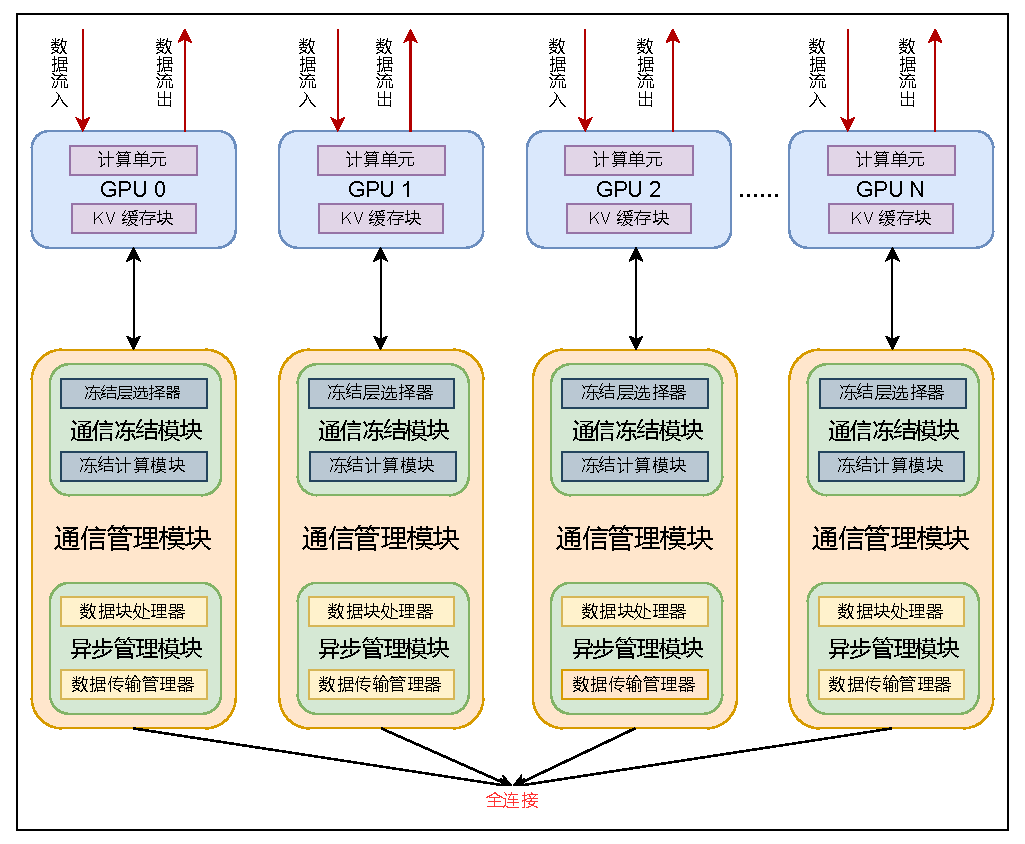
\includegraphics[width=\linewidth]{framework.pdf}
    \caption{整体架构示意图}
    \label{fig:framework}
\end{figure}

\par
新通信管理模块通过以下三个核心组件实现优化:
\begin{itemize}
    \item \textbf{通信冻结模块}:包含冻结层选择器与冻结计算模块。选择器基于KV矩阵相似度(余弦相似度)、
    特征图相似性(L2距离)及冻结历史等多维度指标,动态筛选可冻结层。计算单元根据选择结果执行节点分配策略,
    通过增量更新KV缓存和跨GPU特征复用,降低通信开销。
    \item \textbf{异步通信模块}:由数据块处理器与传输管理器构成。处理器根据实时通信负载状态,
    采用自适应分片算法将数据包划分为细颗粒度的通信包。传输管理器结合冻结节点状态,
    对细粒度数据包执行优先级调度和异步传输。
    \item \textbf{GPU推理模块}:保留核心计算单元,通过缓存机制为冻结节点提供跨GPU的图像数据与KV矩阵缓存。
    在数据流处理过程中,实现计算与通信的并行操作,隐藏通信延迟。
\end{itemize}

\subsection{通信冻结模块}
\label{subsubsec:通信冻结模块}
\subsubsection{图像质量与通信冻结平衡}
\label{subsubsec:图像质量与通信冻结平衡}
在进行通信冻结时,需要在降低通信开销与保持生成图像质量之间取得平衡。为深入探究通信冻结对图像质量的影响,
本节测试了两种常见的固定冻结策略,并结合定量指标(如 PSNR 和 FID等)进行分析。

\begin{itemize}
    \item \textbf{连续冻结同一层}:设置固定冻结层为第 $l$ 层,在分布式推理过程中连续冻结该层,
    并观察冻结前后的图像质量变化,如\autoref{fig:freeze-consecutive}所示。
    \begin{figure}[ht]
        \centering
        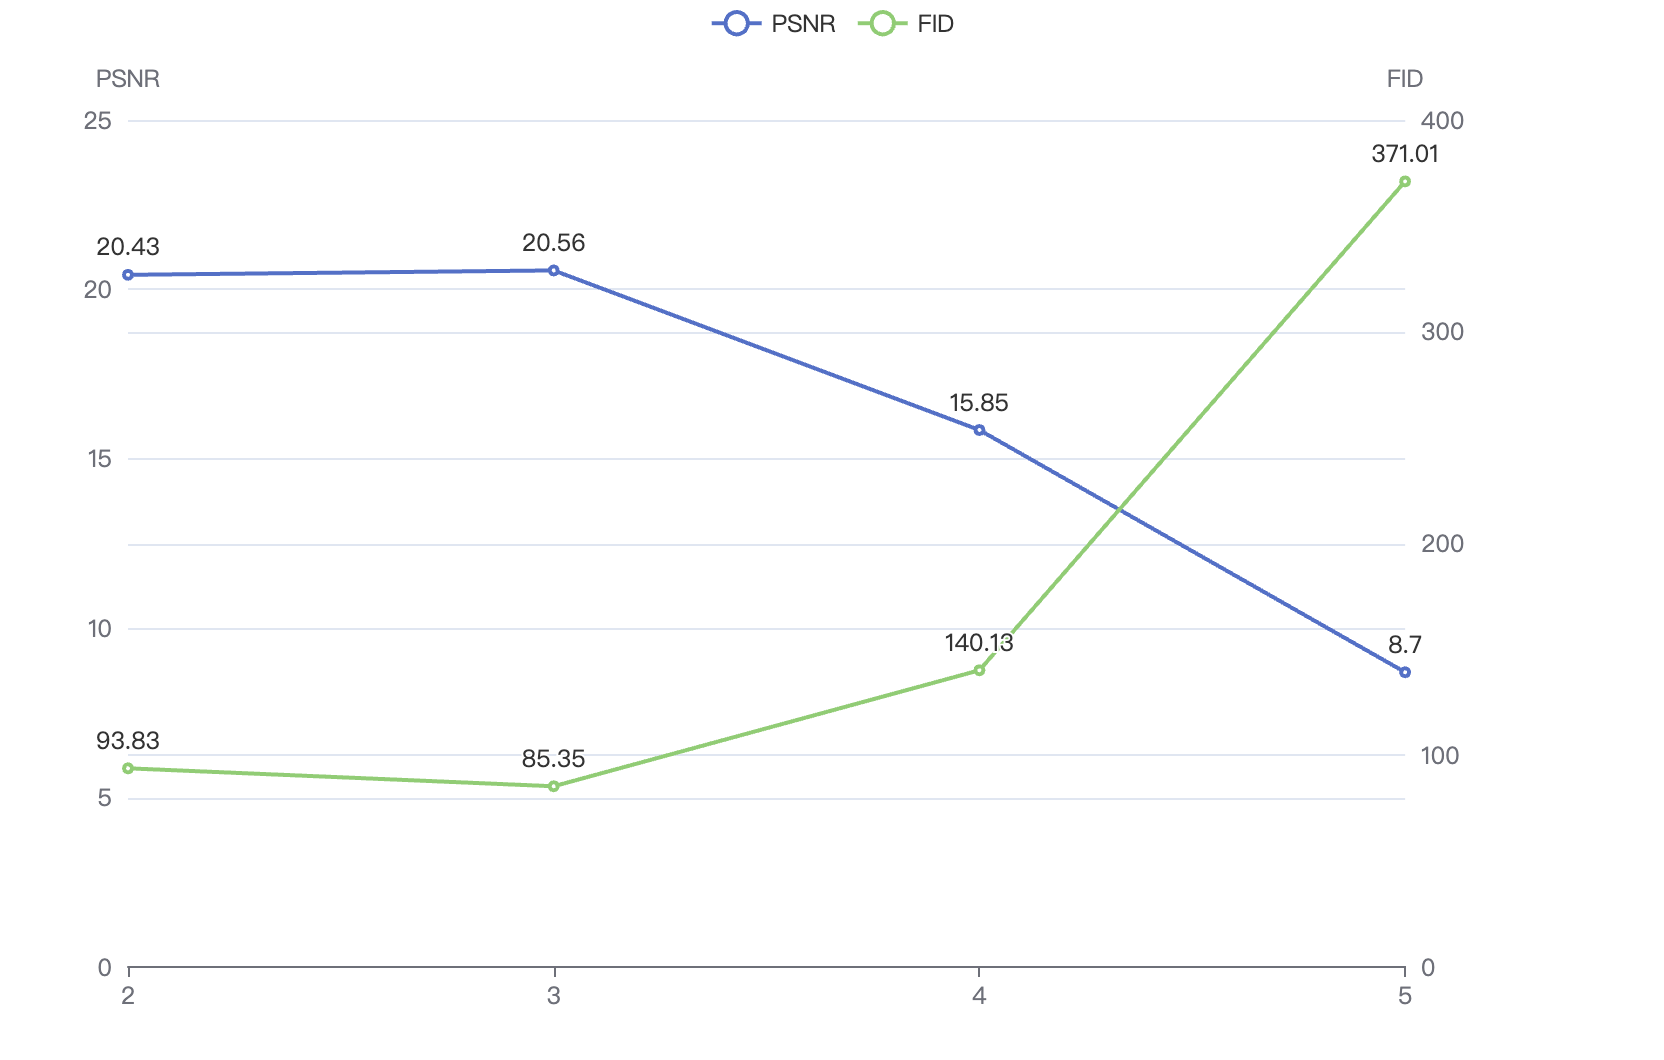
\includegraphics[width=0.8\linewidth]{freeze-consecutive.png}
        \caption{连续冻结同一层对图像质量的影响}
        \label{fig:freeze-consecutive}
    \end{figure}
    实验结果显示,随着连续冻结次数增加,图像质量逐渐下降。例如,当连续冻结 4 次时,PSNR降低至8.7,图片质量较低
    同时可以看到,连续冻结超过 3 次后,PSNR 明显下降,FID 快速上升,视觉感知质量显著恶化。
    因此,在制定冻结策略时应避免对同一层进行多次连续冻结。
    \item \textbf{选择固定数量冻结层}:设置冻结层数量为固定值(如每次冻结10层、20 层等),
    在分布式推理过程中冻结相应数量的层,并观察图像质量的变化趋势,如\autoref{fig:freeze-fixed}所示。
    \begin{figure}[ht]
        \centering
        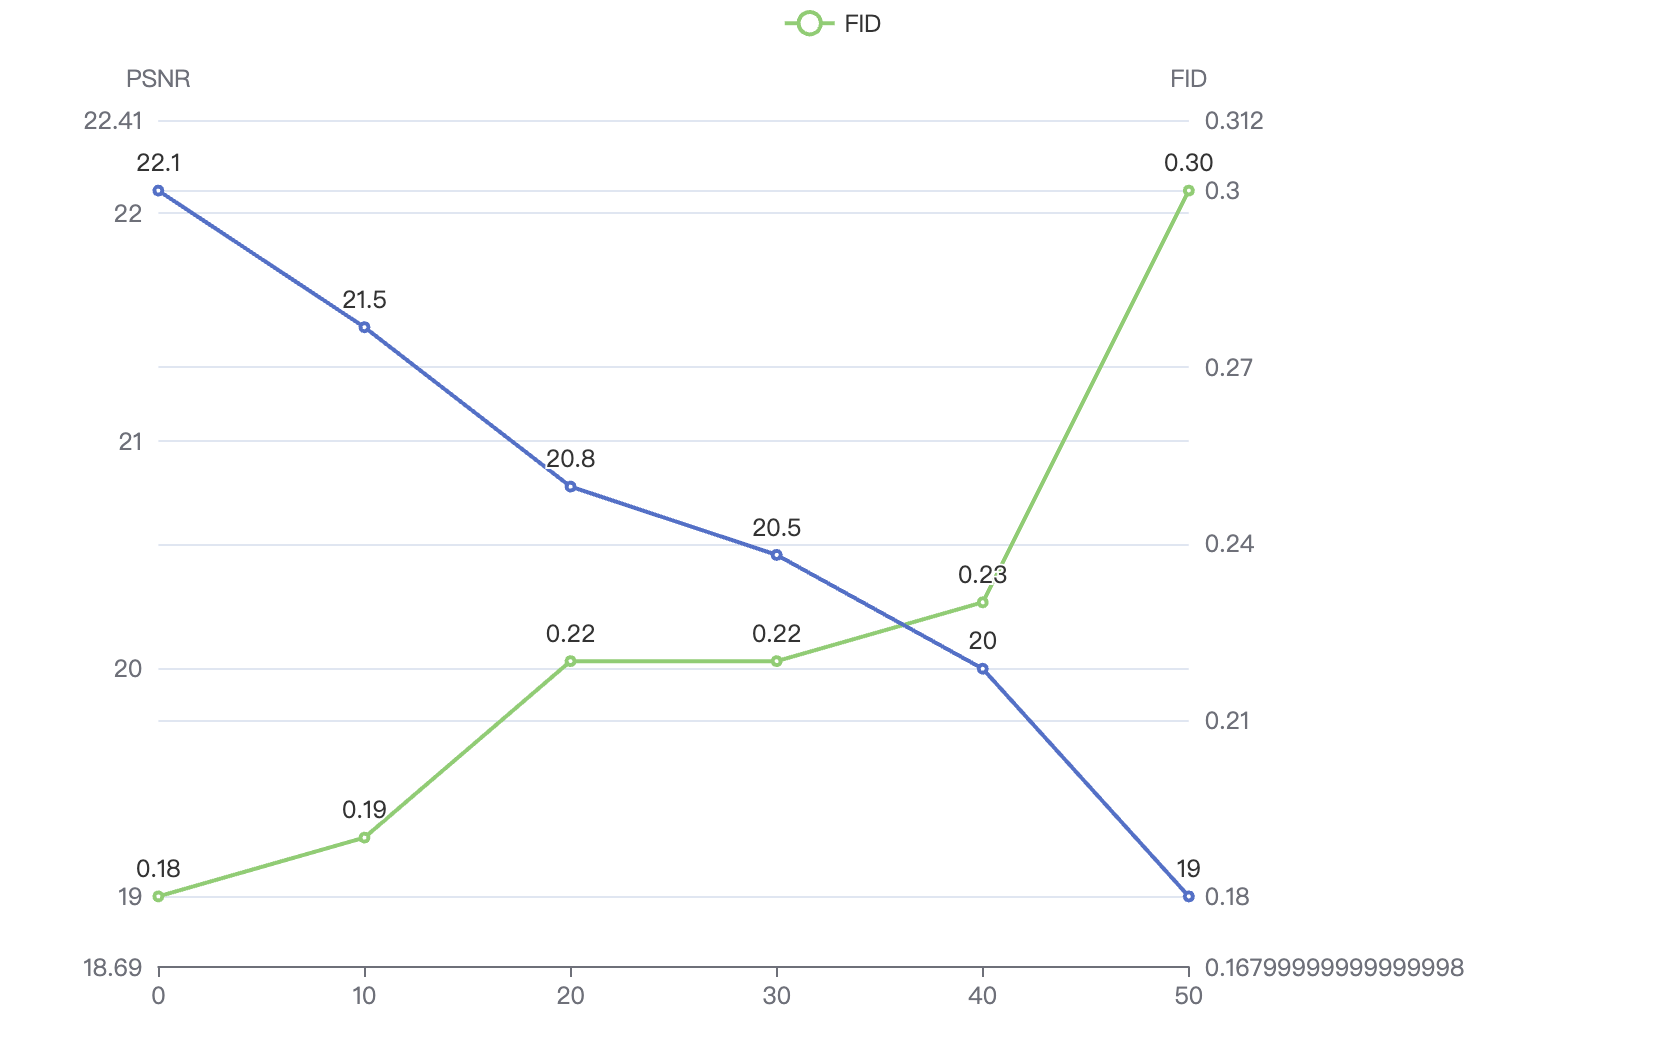
\includegraphics[width=0.8\linewidth]{freeze-fixed.png}
        \caption{选择固定数量冻结层对图像质量影响}
        \label{fig:freeze-fixed}
    \end{figure}
    实验数据显示,随着冻结层数的增加,图像质量呈稳定下降趋势。
    这表明,固定的冻结策略虽然便于实现,但会不可避免地导致图像质量下降。尤其在冻结层数较多时,
    模型的表达能力受限,细节丢失明显。
\end{itemize}
\par
上述实验表明,固定冻结策略会对图像质量造成负面影响,尤其是连续冻结某一层或大量冻结多层时更为明显。
因此,在实际应用中,应采用更加灵活的动态冻结策略,根据每一步的 KV 缓存相似度自适应选择冻结对象,
从而在保证图像质量的前提下优化通信效率。

\subsubsection{冻结层选择器}
\par
基于\ref{sec:diffusion_model_inference_process_similarity}节的研究,扩散模型在推理阶段的相邻步骤中,KV缓存(Key-Value Cache)的相似性整体较高但存在差异。
针对这一特性,可以为每一层定义一个可冻结度指标,其计算公式如下:
\begin{equation}
    F_l = \frac{1 + \text{CosSim}(\mathbf{K}_t^{(l)}, \mathbf{K}_{t-1}^{(l)})}{2}
\end{equation}
其中:
\begin{equation}
    \text{CosSim}(\mathbf{K}_t^{(l)}, \mathbf{K}_{t-1}^{(l)}) = 
    \frac{
        \text{vec}(\mathbf{K}_t^{(l)})^\top \cdot \text{vec}(\mathbf{K}_{t-1}^{(l)})
    }{
        \left\|\text{vec}(\mathbf{K}_t^{(l)})\right\|_2 \cdot \left\|\text{vec}(\mathbf{K}_{t-1}^{(l)})\right\|_2
    }
\end{equation}
\par
\begin{itemize}
    \item $F_l$:第 $l$ 层的可冻结度;
    \item $\mathbf{K}_t^{(l)}$:第 $t$ 步第 $l$ 层的 KV 缓存矩阵;
    \item $\mathbf{K}_{t-1}^{(l)}$:第 $t - 1$ 步第 $l$ 层的 KV 缓存矩阵;
    \item $\|\cdot\|_2$:向量的 L2 范数。
\end{itemize}
\par
计算后,通过 $(1 + \cdot)/2$ 操作将相似度映射到 [0, 1] 区间,便于后续比较和阈值设定。
总体来讲,相似性越高,$F_l$ 越接近 1,
表明该层更适合作为冻结对象。
\par
计算相似度后,通过维护一个可冻结度数组 $[F_1, F_2, \dots, F_L]$,对所有层进行排序并动态更新。
最后根据初始化的阈值 $\theta$ 选择可冻结层,并返回结果。
具体算法伪代码如算法\ref{alg:freeze_selector}。
\begin{algorithm}[!h]
    \caption{冻结层选择算法}
    \label{alg:freeze_selector}
    \renewcommand{\algorithmicrequire}{\textbf{Input:}}
    \renewcommand{\algorithmicensure}{\textbf{Output:}}
    \begin{algorithmic}[1]
        \REQUIRE 模型层数 $L$,KV缓存序列 $\{\mathbf{K}_t^{(l)}\}$,阈值 $\theta$
        \ENSURE 冻结层集合 $\text{frozen\_layers}$
        \STATE Initialize $\text{freezability\_scores} \leftarrow [0]^L$
        \FOR{$l = 1$ to $L$}
            \STATE $\text{freezability\_scores}[l] \leftarrow \frac{1 + \text{CosSim}(\mathbf{K}_t^{(l)}, \mathbf{K}_{t-1}^{(l)})}{2}$
        \ENDFOR
        \STATE $\text{sorted\_indices} \leftarrow \text{argsort}(\text{freezability\_scores})$ 
        \STATE $\text{frozen\_layers} \leftarrow \emptyset$
        \FOR{$idx \in \text{sorted\_indices}$}
            \IF{$\text{freezability\_scores}[idx] > \theta$}
                \STATE $\text{frozen\_layers} \leftarrow \text{frozen\_layers} \cup \{idx\}$
                \STATE \textbf{break}
            \ENDIF
        \ENDFOR
        \RETURN $\text{frozen\_layers}$
    \end{algorithmic}
\end{algorithm}
\par
使用上述方法后,实验发现图像质量会出现显著下降问题,经具体研究发现由于部分层的KV缓存相似度始终较高,导致其一直处于冻结
状态,产生了误差累积。因此,需要设置另一个参数来记录每层的冻结历史情况,综合KV缓存相似度和冻结历史情况,来确定该层是否
应该被冻结,优化后的公式如下:
\begin{equation}
    F_l' = F_l \times \left(1 - \frac{c_l}{c_{\text{max}}}\right)
\end{equation}
\par
其中:
\begin{itemize}
    \item $F_l$:第 $l$ 层的原始可冻结度;
    \item $c_l$:第 $l$ 层的冻结计数器;
    \item $c_{\text{max}}$:最大冻结次数阈值;
    \item $F_l'$:第 $l$ 层优化后的可冻结度。
\end{itemize}
\par
当某层的被冻结后,$c_l$增大时,$F_l'$降低,从而抑制频繁冻结。结合优化可冻结度公式
后的算法如算法\ref{alg:freeze_selector_v2}所示:
\begin{algorithm}[!h]
    \caption{优化后的冻结层选择算法}
    \label{alg:freeze_selector_v2}
    \renewcommand{\algorithmicrequire}{\textbf{Input:}}
    \renewcommand{\algorithmicensure}{\textbf{Output:}}
    \begin{algorithmic}[1]
        \REQUIRE 模型层数 $L$,KV缓存序列 $\{\mathbf{K}_t^{(l)}\}$,阈值 $\theta$,最大冻结次数 $c_{\text{max}}$
        \ENSURE 冻结层集合 $\text{frozen\_layers}$
        \STATE Initialize $\text{freezability\_scores} \leftarrow [0]^L$
        \STATE Initialize $\text{freeze\_count} \leftarrow [0]^L$ 
        \FOR{$l = 1$ to $L$}
            \STATE $F_l \leftarrow \frac{1 + \text{CosSim}(\mathbf{K}_t^{(l)}, \mathbf{K}_{t-1}^{(l)})}{2}$
            \STATE $\text{decay} \leftarrow 1 - \min(\text{freeze\_count}[l], c_{\text{max}}) / c_{\text{max}}$
            \STATE $\text{freezability\_scores}[l] \leftarrow F_l \times \text{decay}$
        \ENDFOR
        \STATE $\text{sorted\_indices} \leftarrow \text{argsort}(\text{freezability\_scores})$ 
        \STATE $\text{frozen\_layers} \leftarrow \emptyset$
        \FOR{$idx \in \text{sorted\_indices}$}
            \IF{$\text{freezability\_scores}[idx] > \theta$}
                \STATE $\text{frozen\_layers} \leftarrow \text{frozen\_layers} \cup \{idx\}$
                \STATE $\text{freeze\_count}[idx] \leftarrow \text{freeze\_count}[idx] + 1$ 
                \STATE \textbf{break}
            \ENDIF
        \ENDFOR
        \RETURN $\text{frozen\_layers}$
    \end{algorithmic}
\end{algorithm}

\subsubsection{冻结计算模块}
由\ref{sec:diffusion_model_distributed_inference_communication_delay}节的研究可知,现有扩散模型分布式推理框架中存在严重的通信延迟问题,导致 GPU 在等待数据传输期间处于空闲状态,
浪费了很多计算资源。为缓解这一问题设计冻结计算模块,其核心思想是:在 GPU 执行计算任务的同时完成通信操作,
从而实现计算与通信的重叠,提高整体效率。
为此,我们需要根据当前步骤的 GPU 计算时间 $t_{\text{comp}}$ 和通信时间 $t_{\text{comm}}$,
动态计算在 GPU 计算期间最多可以完成的可节省的最大通信数据量 $\Delta V$,即:
\begin{equation}
    \Delta V = V_{\text{total}} \times \left( \frac{t_{\text{comm}}}{t_{\text{comp}}} - 1 \right)
\end{equation}
其中:
\begin{itemize}
    \item $V_{\text{total}}$:当前步骤的总通信数据量;
    \item $t_{\text{comm}}$:当前步骤的通信耗时;
    \item $t_{\text{comp}}$:当前步骤的 GPU 计算耗时。
\end{itemize}
\par
通过该公式可得,在不影响整体执行效率的前提下,系统最多可以减少 $\Delta V$ 的通信数据量。根据可减少的最大通信数据量
以及冻结层选择器传入的可冻结层序列,依次选取序列中的可冻结层直到累积通信数据量 $\geq \Delta V$ ,然后对已经选取
的可冻结层进行通信冻结,在接下来的步骤中对这些层使用缓存中的旧数据,而不使用通信更新的数据。
\par
同时,结合\ref{subsubsec:图像质量与通信冻结平衡}节的分析,除了考虑可减少的最大通信数据量以及可冻结层序列之外,冻结总数应限制在一定范围内,为了保持
图像质量,根据\autoref{fig:freeze-fixed}的数据,应该设置最大冻结层数(如:50层)来平衡图像质量和通信延迟。如
算法\ref{alg:freeze_selector_communication_aware}所示:
\begin{algorithm}[!h]
    \caption{基于通信优化的冻结层选择算法}
    \label{alg:freeze_selector_communication_aware}
    \renewcommand{\algorithmicrequire}{\textbf{Input:}}
    \renewcommand{\algorithmicensure}{\textbf{Output:}}
    \begin{algorithmic}[1]
        \REQUIRE 
            可冻结层序列 $\text{layers} = [l_1, l_2, ..., l_N]$,
            每层通信数据量 $\text{comm\_volume}[l], \forall l \in \text{layers}$,
            可减少的最大通信数据目标 $\Delta V$,
            最大冻结层数 $f_{\text{max}}$
        \ENSURE 冻结层集合 $\text{frozen\_layers}$
        
        \STATE Initialize $\text{frozen\_layers} \leftarrow \emptyset$
        \STATE Initialize $\text{cumulative\_reduction} \leftarrow 0$
        \STATE Initialize $\text{frozen\_count} \leftarrow 0$

        \FOR{$l \in \text{layers}$}
            \IF{$\text{cumulative\_reduction} + \text{comm\_volume}[l] > \Delta V$ \OR $\text{frozen\_count} \geq f_{\text{max}}$}
                \STATE \textbf{break}
            \ENDIF
            \STATE $\text{frozen\_layers} \leftarrow \text{frozen\_layers} \cup \{l\}$
            \STATE $\text{cumulative\_reduction} \leftarrow \text{cumulative\_reduction} + \text{comm\_volume}[l]$
            \STATE $\text{frozen\_count} \leftarrow \text{frozen\_count} + 1$
        \ENDFOR
        
        \RETURN $\text{frozen\_layers}$
    \end{algorithmic}
\end{algorithm}

\subsection{异步通信模块}

基于对通信冻结模块(见 \ref{subsubsec:通信冻结模块} 节)的研究与测试,我们了解到为确保图像质量下降在可接受范围内,
通信冻结程度存在上限。尽管使用通信冻结模块进行了一定程度的通信优化,但在整个推理过程中仍不可避免地存在通信延迟。
为此,设计了一个异步通信模块以细粒度控制数据传输,从而达到计算-通信隐藏的效果。
\par
在Distrifusion分布式推理框架中,数据块采用All-Gather方法进行传输(具体传输方式参见
\ref{sec:pytorch-communication}节)。在每次推理迭代中,Distrifusion利用checkpoint机制累积数据块,
当累积的数据块数量达到$N_{\text{chk}}$(例如$N_{\text{chk}}=60$)时,将所有数据聚合后一次性传输。
这种做法导致每次数据传输量较大,在计算完成之后数据传输尚未结束,从而引入了显著的通信延迟\cite{li2024distrifusion}。
\par
为了解决这一问题,我们将数据划分为更小的部分进行传输。首先尝试最简单的方法,即每当获得一个数据块就立即传输。
然而,实际测试表明,这种方法由于频繁建立NCCL All-Gather通信连接,其建立连接的时间开销远大于直接的通信延迟,
反而降低了整体效率。
因此,我们需要找到一种自适应的数据块划分策略,既能实现异步传输效果,又能避免过于频繁地建立连接。
这里设定了一个超参数$N_{\text{chk}}$作为单次All-Gather操作的数据包大小,
并通过实验确定最佳的$N_{\text{chk}}$值,以平衡传输效率与连接开销。这里使用网格搜索法得到最优参数,
在预定义的范围内等间距地选取多个候选值,分别测试性能,最后选择最优数据包大小。具体算法
如\ref{alg:grid_search_packet_size}。
\begin{algorithm}[!h]
    \caption{基于网格搜索的最优数据包大小选择算法}
    \label{alg:grid_search_packet_size}
    \renewcommand{\algorithmicrequire}{\textbf{Input:}}
    \renewcommand{\algorithmicensure}{\textbf{Output:}}
    \begin{algorithmic}[1]
        \REQUIRE 
            候选数据包大小集合 $\mathcal{S} = \{s_1, s_2, ..., s_N\}$,  
            测试迭代次数 $T$,
            性能评估函数 $\text{measure\_performance}(S_{\text{packet}})$
        \ENSURE 最优数据包大小 $S^*$
        \STATE Initialize $\text{best\_score} \leftarrow +\infty$
        \STATE Initialize $\text{best\_packet\_size} \leftarrow \text{None}$
        \FOR{$s \in \mathcal{S}$}
            \STATE $\text{avg\_latency} \leftarrow 0$
            \FOR{$t = 1$ to $T$}
                \STATE $\text{latency} \leftarrow \text{measure\_performance}(s)$
                \STATE $\text{avg\_latency} \leftarrow \text{avg\_latency} + \text{latency} / T$
            \ENDFOR
            \IF{$\text{avg\_latency} < \text{best\_score}$}
                \STATE $\text{best\_score} \leftarrow \text{avg\_latency}$
                \STATE $\text{best\_packet\_size} \leftarrow s$
            \ENDIF
        \ENDFOR
        \RETURN $\text{best\_packet\_size}$
    \end{algorithmic}
\end{algorithm}
\par
最终,Distrifusion推理框架、简单方法、最优数据包三种方法的通信与计算对比如下所示:
\begin{figure}[ht]
    \centering
    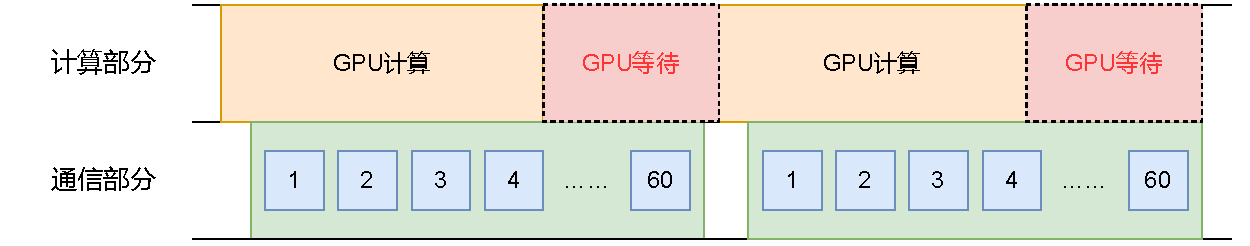
\includegraphics[width=0.9\linewidth]{Distrifusion-compute-communication.pdf}
    \caption{Distrifusion框架计算与通信过程}
    \label{fig:Distrifusion-compute-communication}
\end{figure}
\begin{figure}[ht]
    \centering
    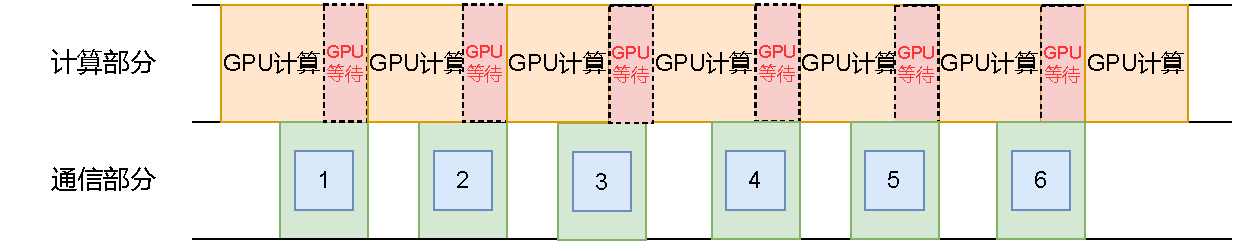
\includegraphics[width=0.9\linewidth]{Native-compute-communication.pdf}
    \caption{简单分块方法计算与通信过程}
    \label{fig:Native-compute-communication}
\end{figure}
\begin{figure}[ht]
    \centering
    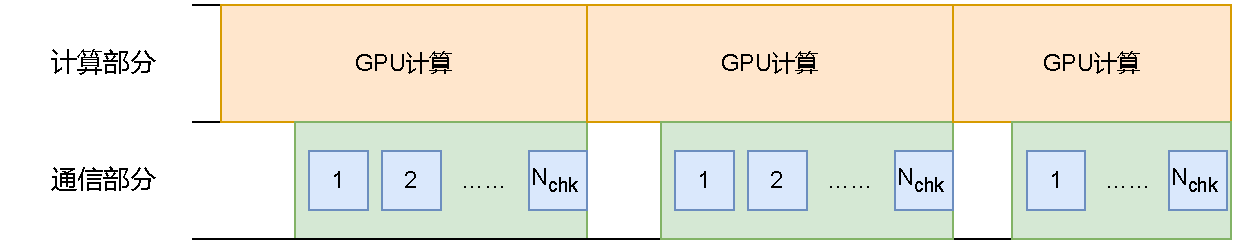
\includegraphics[width=0.8\linewidth]{our-compute-communication.pdf}
    \caption{本文方法计算与通信过程}
    \label{fig:our-compute-communication}
\end{figure}
\par
通过比较分析,可以直观地看到不同方法在通信与计算过程中的表现差异。
\begin{itemize}
    \item \textbf{Distrifusion推理框架:}如\autoref{fig:Distrifusion-compute-communication}所示,
    Distrifusion框架当累积的数据块数量达到$N_{\text{chk}}=60$)时,所有数据被聚合并一次性传输。虽然简化了
    通信管理,但由于每次传输的数据量较大,导致在计算完成后,数据传输往往尚未结束,从而引入了显著的通信延迟。这种延
    迟限制了系统的整体效率,尤其是在低带宽GPU互连集群中。
    \item \textbf{简单分块方法:}相比之下,\autoref{fig:Native-compute-communication}展示了简单分块方法
    的执行流程。这种方法尝试将数据块直接传输来缓解大块数据传输带来的延迟问题。然而,
    频繁建立通信连接的时间开销在累积后远大于直接的通信延迟。
    这意味着尽管这种方法旨在减少传输延迟,但实际上却因额外的连接时间而降低了整体效率,特别是在高性能计算环境中,
    这种额外的开销是不可接受的。
    \item \textbf{本文提出的方法:}
    \autoref{fig:our-compute-communication}呈现了本文提出的优化方法。
    该方法利用网格搜索等技术确定最佳参数后自适应地选择最优的数据包大小$N_{\text{chk}}$,
    实现了通信与计算的有效重叠。
\end{itemize}
\par
综上所述,本文的方法能够在低成本商用GPU(如RTX4090)上实现高效的异步通信。这不仅减少了不必要的连接开销,
还确保了通信与计算的高效并行,从而提升了系统整体性能。实验结果表明,
相较于前两种方法,本文的方法在保持良好图像质量的同时,显著降低了通信延迟,提高了分布式推理的效率。

\section{实验环境及配置}
\label{sec:exp-env}
在具体实验测试中,构建了完备的硬件测试环境,包含PCIe与NVLink两种典型互连架构的GPU集群。
配置多卡并行训练场景来验证分布式框架在不同计算场景下的适应性。具体实验环境及配置如下:
\begin{itemize}
    \item \textbf{硬件配置}:实验采用两种异构计算集群进行对比测试:
    \begin{itemize}
        \item [(1)] NVIDIA RTX 4090,配备2颗Intel Xeon Gold 6130处理器及256GB DDR4内存,
        通过PCIe 3.0总线实现多卡互联\cite{IntelXeonGold,A100};
        \item [(2)] NVIDIA A100,配备2颗Intel Xeon Gold 6130处理器与256GB DDR4内存,
        利用NVLink实现GPU间高速互连,带宽为80GB/s\cite{IntelXeonGold, RTX4090}。
    \end{itemize}
    \item \textbf{软件环境}:系统构建于PyTorch 2.4深度学习框架\cite{PyTorch2.4},搭配Python 3.11解释器与CUDA 12.1计算架构。
    利用huggingface diffusers 0.24.0库实现基础扩散模型\cite{huggingface},分布式通信层采用NCCL后端,
    通过torch.distributed模块实现跨节点并行控制。
    \item \textbf{测试配置}:在1/2/4/8 GPU不同规模下进行对比实验,重点考察两种互连架构的性能表现。
\end{itemize}

\section{实验结果分析}
\subsection{实验对象及测试指标}
\label{sec:experiment-object}
\par
本文的实验使用典型图像生成扩散模型模型 —— Stable Diffusion XL(简称 SDXL),SDXL 是目前广泛使用、
性能优异的扩散模型,且已经进行了代码开源,适合进行系统性优化研究\cite{Podell2023SDXLIL}。同时,我们使用COCO
图像-提示词数据集进行测试,该数据集包含了超过 150 万条提示词及 33 万张常见图像,经常用来做视觉模型的基准测试
\cite{Chen2015MicrosoftCC}。
\par
在实验中,具体测试的指标主要有:
\begin{itemize}
    \item \textbf{推理延迟}:测试从输入文本开始,到模型生成完整图像所需的总时间。在测试总推理延迟的同时,
    分别测试\textbf{通信延迟}与\textbf{计算延迟},用于更好地评估本文推理框架的具体效果。
    \item \textbf{图像质量}:为了方便与Distrifusion框架进行对比,沿用其图像质量测试指标,包括PSNR(越高图像质量越好)、
    LPIPS(越低图像质量越好)、FID(越低图像质量越好)。具体指标含义见\ref{sec:image-quality-metric}。
\end{itemize}
综上,本文从两个方面评估推理框架的性能:一是端到端的文本到图像生成延迟,
二是图像质量,后者通过 PSNR、LPIPS 和 FID 三个标准指标进行综合评估,
从而全面验证系统在加速推理的同时是否保持了良好的生成效果。

\subsection{实验测试方法}
\label{sec:experiment-method}
为了测试推理框架的优化性能,本文将优化后的推理框架与基础分布式推理模型、Distrifusion框架、随机优化方法、简化优化方法
进行了全面测试与对比,方法详细解释如下:
\begin{itemize}
    \item \textbf{基础分布式推理模型(Native)}:使用同步通信(计算与通信分离)的基础分布式模型,
    作为测试的基准框架。
    \item \textbf{Distrifusion框架(Distrifusion)}:目前最前沿扩散模型的分布式推理框架,使用缓存来进行通信优化
    \cite{li2024distrifusion}。
    \item \textbf{随机优化方法(Random)}:在\ref{subsubsec:通信冻结模块}节
    基础上使用随机冻结注意力层的推理方式,以 50\% 的概率随机决定是否冻结可冻结层;
    \item \textbf{简化优化方法(Simplified)}:在\ref{subsubsec:通信冻结模块}节
    基础上冻结所有可冻结层,极大程度上消除通信(但会影响图像质量);
    \item \textbf{优化方法(our's)}:本文优化方法,在保证图像质量的基础上进行通信优化。
\end{itemize}
\par
后续测试图表中均使用括号内的英文简称作为图例使用。
\subsection{实验结果及分析}
\subsubsection{主要实验结果}
\label{sec:main-experiment-result}
\par
根据 \ref{sec:experiment-object} 节的测试对象及 \ref{sec:experiment-method} 节的测试方法,
本研究针对典型高分辨率图像(1024×1024、1536×1536)开展了分布式推理性能评估。为验证低成本商用 GPU 集群
通过 PCIe 互联的实际表现,采用 4/8 卡 RTX 4090 GPU 构建测试环境,重点对比基础模型与优化方法在延迟与质量
方面的差异。实验结果如下:
\par
\textbf{(1)推理延迟对比}:
\begin{itemize}
    \item 在 1024×1024 分辨率下,4/8 GPU 集群对基础分布式模型、DistriFusion 框架、随机优化方法、
    简化优化方法及本文优化方法进行了系统测试,结果见图 \ref{fig:experiment-result-1024}。
    \item 在 1536×1536 分辨率下,采用相同测试方法获得对比数据,结果见图 \ref{fig:experiment-result-2048}。
    
    \begin{figure}[ht]
        \centering
        \begin{minipage}[t]{0.45\linewidth}
            \centering
            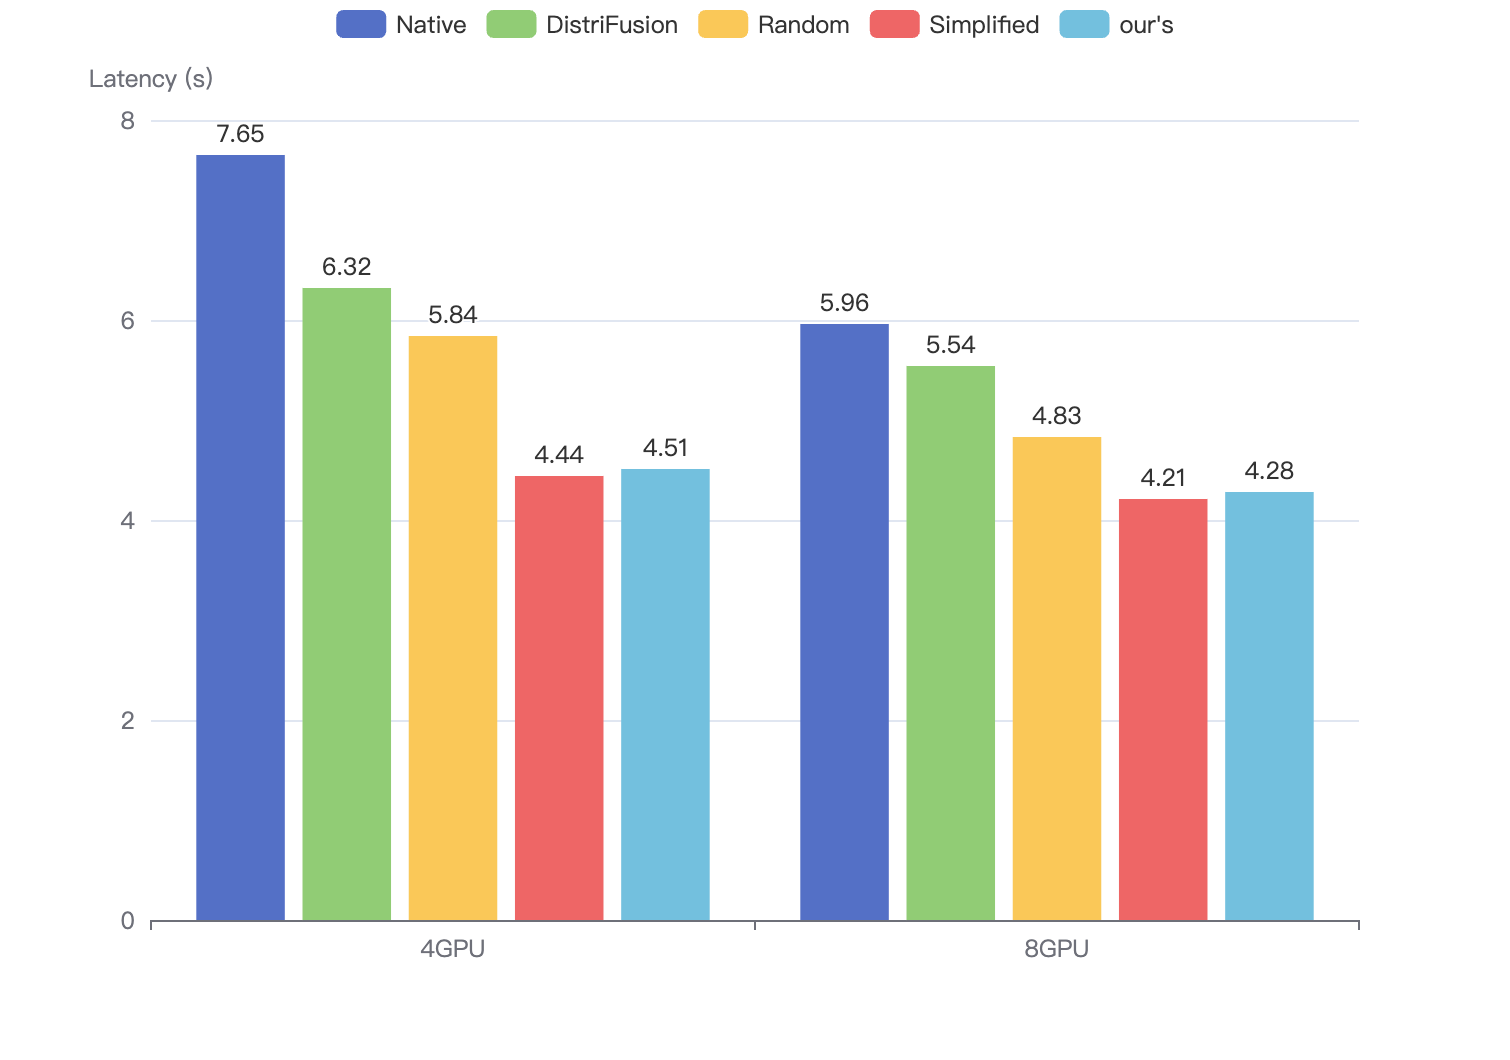
\includegraphics[width=\linewidth]{experiment-result-1024.png}
            \caption{1024×1024 分辨率下各方法推理延迟对比}
            \label{fig:experiment-result-1024}
        \end{minipage}
        \hfill
        \begin{minipage}[t]{0.45\linewidth}
            \centering
            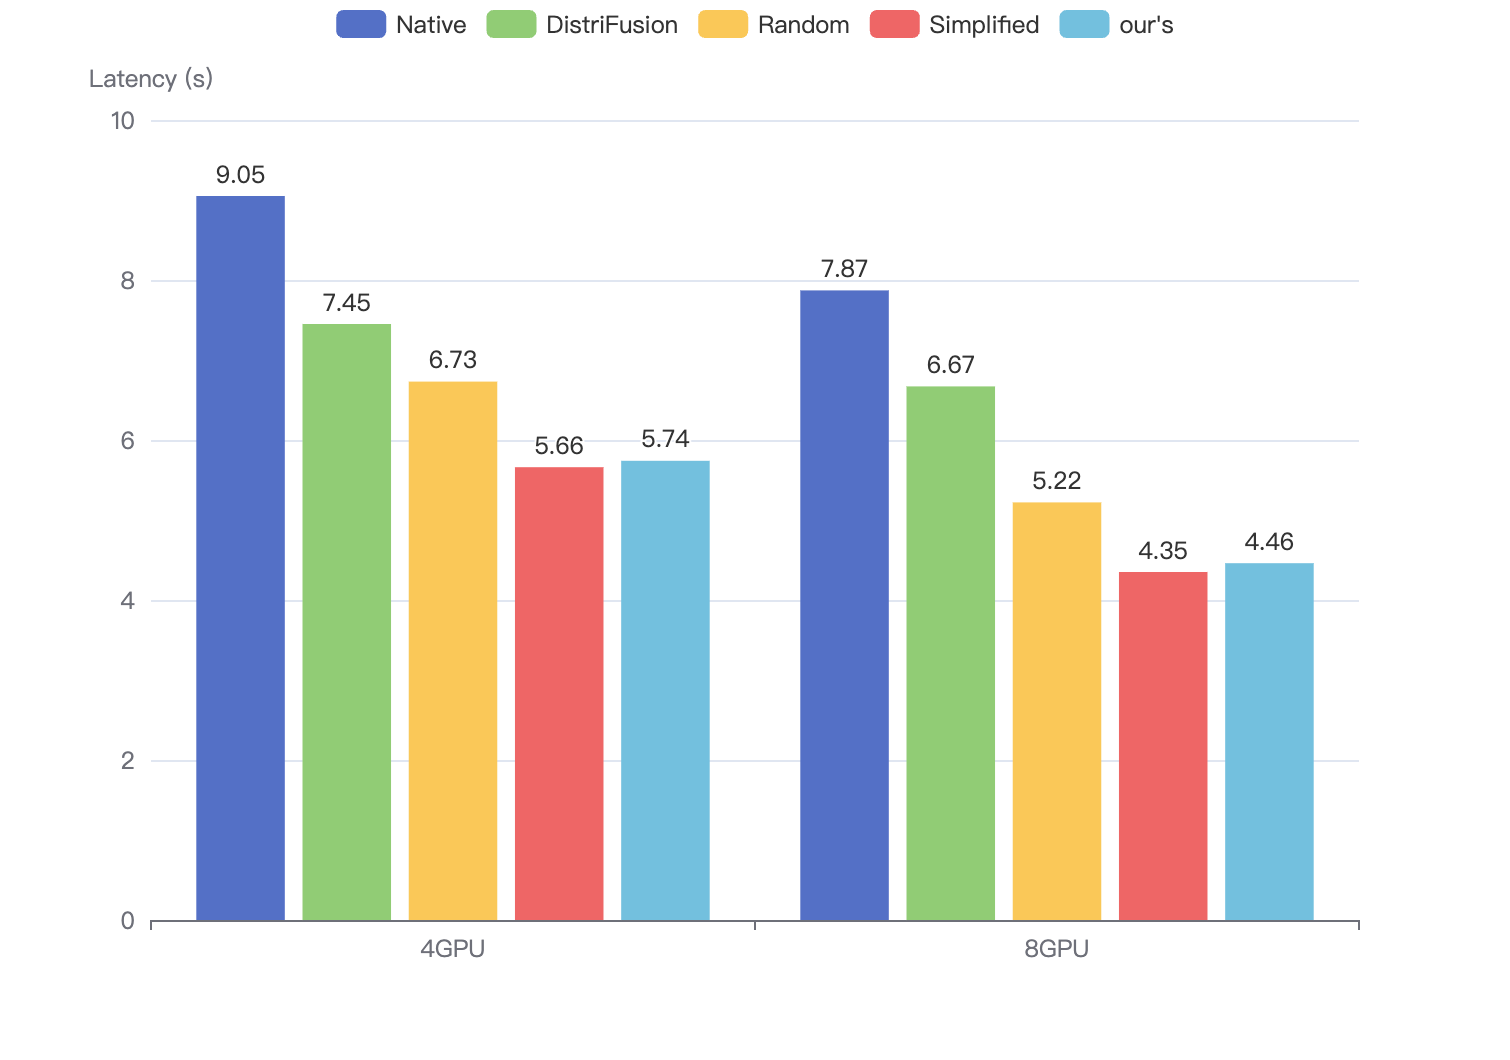
\includegraphics[width=\linewidth]{experiment-result-2048.png}
            \caption{1536×1536 分辨率下各方法推理延迟对比}
            \label{fig:experiment-result-2048}
        \end{minipage}
    \end{figure}
    
    \item 性能分析:
    \begin{enumerate}
        \item 基础分布式模型采用同步通信机制,计算后需等待完整通信过程,通信延迟显著。
        本文方法相比其延迟降低 28\% \~{} 43\%;
        \item DistriFusion 框架通过缓存通信机制实现部分异步通信,仍存在通信等待,
        本文方法延迟降低 23\% \~{} 33\%;
        \item 随机优化方法采用注意力层随机冻结策略,在特定场景易产生冻结错误,稳定性不足。
        本文方法延迟降低 12\% \~{} 23\%;
        \item 简化优化方法通过冻结全部层实现通信延迟消除,虽与本文方法延迟相当,但图像质量明显下降。
    \end{enumerate}
\end{itemize}
\par
因此,本文提出的优化方法在多种高分辨率图像推理场景下均展现出显著的性能优势。相比基础分布式模型,
减少了同步通信带来的等待时间,更好地实现了异步通信效果,在保证图像质量的前提下,有效提升了分布式推理效率,
具有良好的实用性和稳定性。

\par
\textbf{(2)图像质量对比}:
\par
在减小推理延迟的同时,图像质量的性能也十分重要,
因此还需要对各种方法的图像质量进行对比,来验证优化方法的有效性。
下面使用4/8 卡 RTX 4090 GPU集群对\ref{sec:experiment-method} 节的不同测试方法使用
\ref{sec:image-quality-metric} 节中定义的多种指标进行对比,具体结果如表\ref{tab:image-quality-result}所示
(其中,\textbf{w/ G.T.}表示与Ground Truth(图像数据集中的原始图像)进行比较,
而\textbf{w/ Orig.}表示与原始模型生成的图片进行对比)。
生成图片结果(部分示例)如表\ref{tab:image-result}所示。
\begin{table}[ht]
    \centering
    \begin{tabular}{l l c c c c}
    \toprule
    \multirow{2}{*}{GPU数量} & \multirow{2}{*}{推理方法} & \multirow{2}{*}{PSNR ($\uparrow$)} & \multirow{2}{*}{FID ($\downarrow$)} & \multicolumn{2}{c}{LPIPS ($\downarrow$)} \\
    \cmidrule(lr){5-6}
    & & & & w/ G.T. & w/ Orig. \\
    \midrule
    
    \multirow{5}{*}{4}
    & Naive & - & - & 0.798 & - \\
    \cmidrule(lr){2-6}
    & DistriFusion & 23.24 & 24.21 & 0.797 & 0.183 \\
    \cmidrule(lr){2-6}
    & Random & 21.69 & 30.11 & 0.801 & 0.188 \\
    \cmidrule(lr){2-6}
    & Simplified & 19.12 & 55.27 & 0.807 & 0.321 \\
    \cmidrule(lr){2-6}
    & \textbf{our's} & \textbf{22.84} & \textbf{22.83} & \textbf{0.801} & \textbf{0.187} \\
    \midrule
    
    \multirow{5}{*}{8}
    & Naive & - & - & 0.799 & - \\
    \cmidrule(lr){2-6}
    & DistriFusion & 22.06 & 24.41 & 0.799 & 0.209 \\
    \cmidrule(lr){2-6}
    & Random & 20.81 & 29.95 & 0.802 & 0.223 \\
    \cmidrule(lr){2-6}
    & Simplified & 18.38 & 42.17 & 0.806 & 0.381 \\
    \cmidrule(lr){2-6}
    & \textbf{our's} & \textbf{21.91} & \textbf{25.45} & \textbf{0.802} & \textbf{0.211} \\
    \bottomrule
    \end{tabular}
    \caption{不同设备数量下各方法的图像质量对比}
    \label{tab:image-quality-result}
\end{table}

\begin{table}[ht]
    \centering
    \begin{tabular}{cccc}
    \toprule
    DistriFusion & Random & Simplified & our's \\
    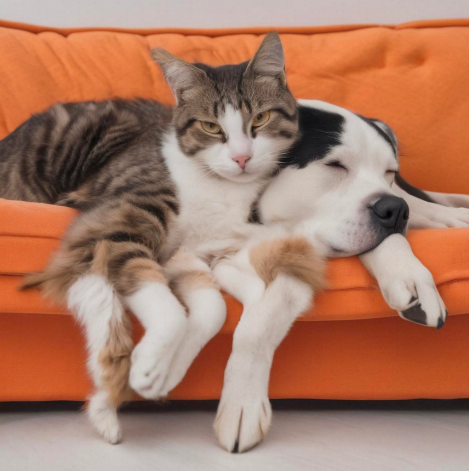
\includegraphics[width=0.23\linewidth]{distrifusion1.png} &
    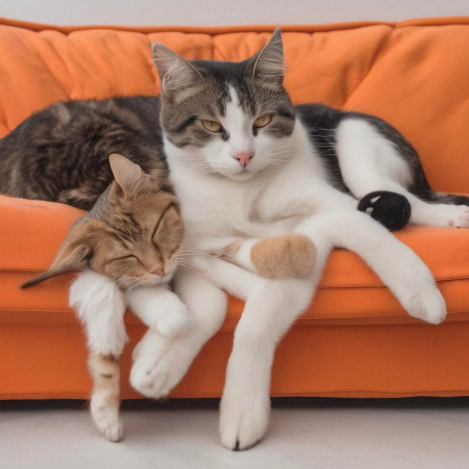
\includegraphics[width=0.23\linewidth]{random1.png} &
    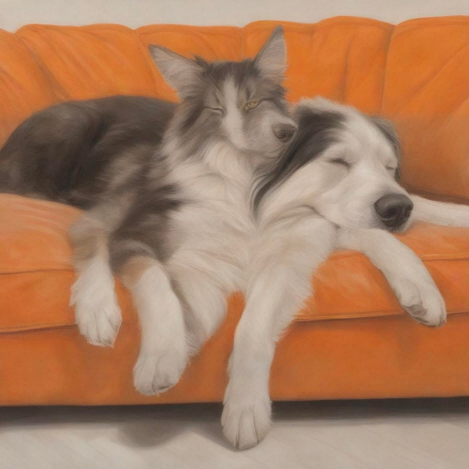
\includegraphics[width=0.23\linewidth]{simplified1.png} &
    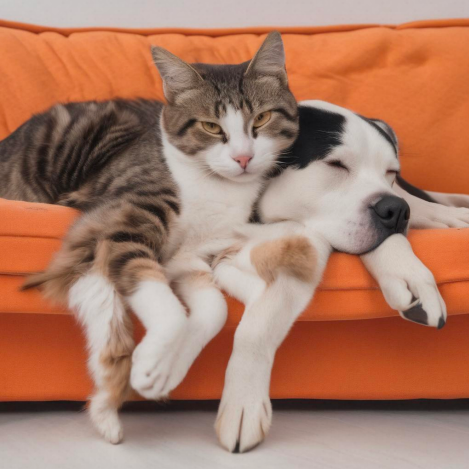
\includegraphics[width=0.23\linewidth]{our1.png} \\
    \multicolumn{4}{c}{输入提示词: A dog and cat are sleeping together on an orange couch.} \\
    \midrule
    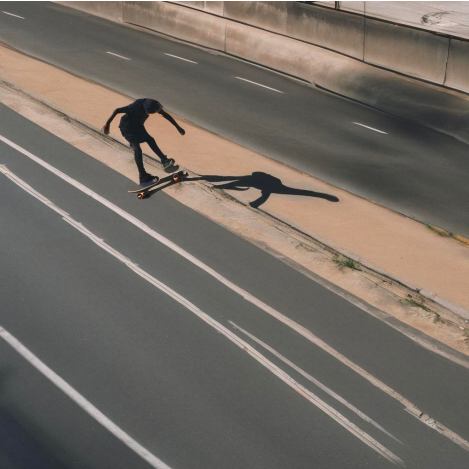
\includegraphics[width=0.23\linewidth]{distrifusion2.png} &
    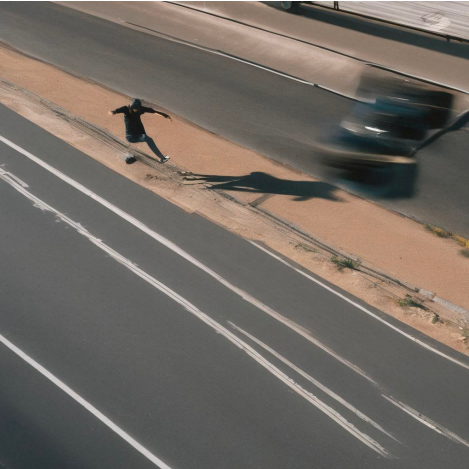
\includegraphics[width=0.23\linewidth]{random2.png} &
    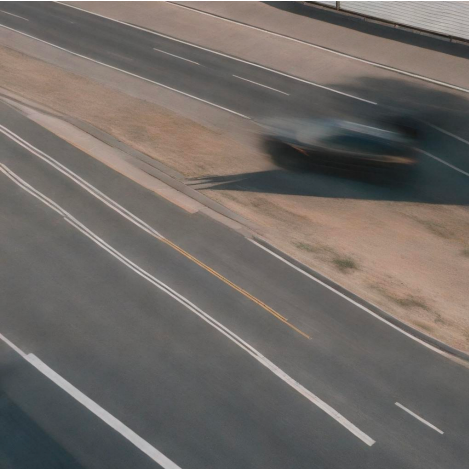
\includegraphics[width=0.23\linewidth]{simplified2.png} &
    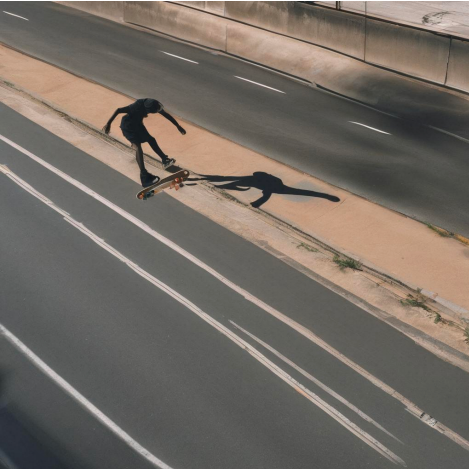
\includegraphics[width=0.23\linewidth]{our2.png} \\
    \multicolumn{4}{c}{输入提示词: A person skateboarding on the side of the road.} \\
    \bottomrule
    \end{tabular}
    \caption{不同方法生成图片结果对比}
    \label{tab:image-result}
\end{table}
\par

实验结果显示,
\begin{itemize}
    \item 本文优化方法与DistriFusion方法相比,FID 明显更低(4 GPU 下低 5.7\%,8 GPU 下低 4\%),
    表明生成图像与真实数据分布更加一致;LPIPS 接近最优值,感知质量稳定;PSNR 略低于 DistriFusion,
    但差距极小(4 GPU 下 降低 0.4,8 GPU 下 降低0.15),且不影响整体质量。
    \item 与Random方法相比,在PSNR、FID、LPIPS 全面优于 Random 方法,尤其 FID 降低约 23\% \~{} 25\%。
    \item 与Simplified方法相比,PSNR、FID、LPIPS 显著优于 Simplified 方法,尤其 FID 降低约 58\% \~{} 59\%。
\end{itemize}
\par
从表\ref{tab:image-result}中可以直观地看出,在不同提示词下生成图片时,DistriFusion框架与本文优化方法
图像清晰度和质量较;,Random方法会出现图像错位(图中小狗的头部错误地生成为小猫头部且位置出现错位)、
部位模糊(滑板部位较模糊)等现象;Simplified方法整体图像十分模糊且混乱,图像质量最低。
\par
由上述分析可知,本文优化方法在图像质量上显著高于Random方法与Simplified方法,基本与DistriFusion方法相似,
在降低推理延迟的同时,保持了高质量的图像生成能力,验证了本文优化策略的平衡性。

\subsubsection{其他配置GPU条件下的性能测试}
\par
本文优化方法主要为了解决传统扩散模型分布式推理框架(如Distrifusion框架)在低成本商用GPU集群下的通信瓶颈问题,在
\ref{sec:main-experiment-result}节中已经证明了优化方法的性能提升,下面将在部署使用 NVLink 技术的GPU 阵列A100
上进行测试对比。本节在不同分辨率以及不同GPU阵列下测试了本文优化方法与Distrifusion框架的推理性能,并进行对比,
具体结果如\autoref{fig:experiment-result-a100}所示。
\begin{figure}[ht]
    \centering
    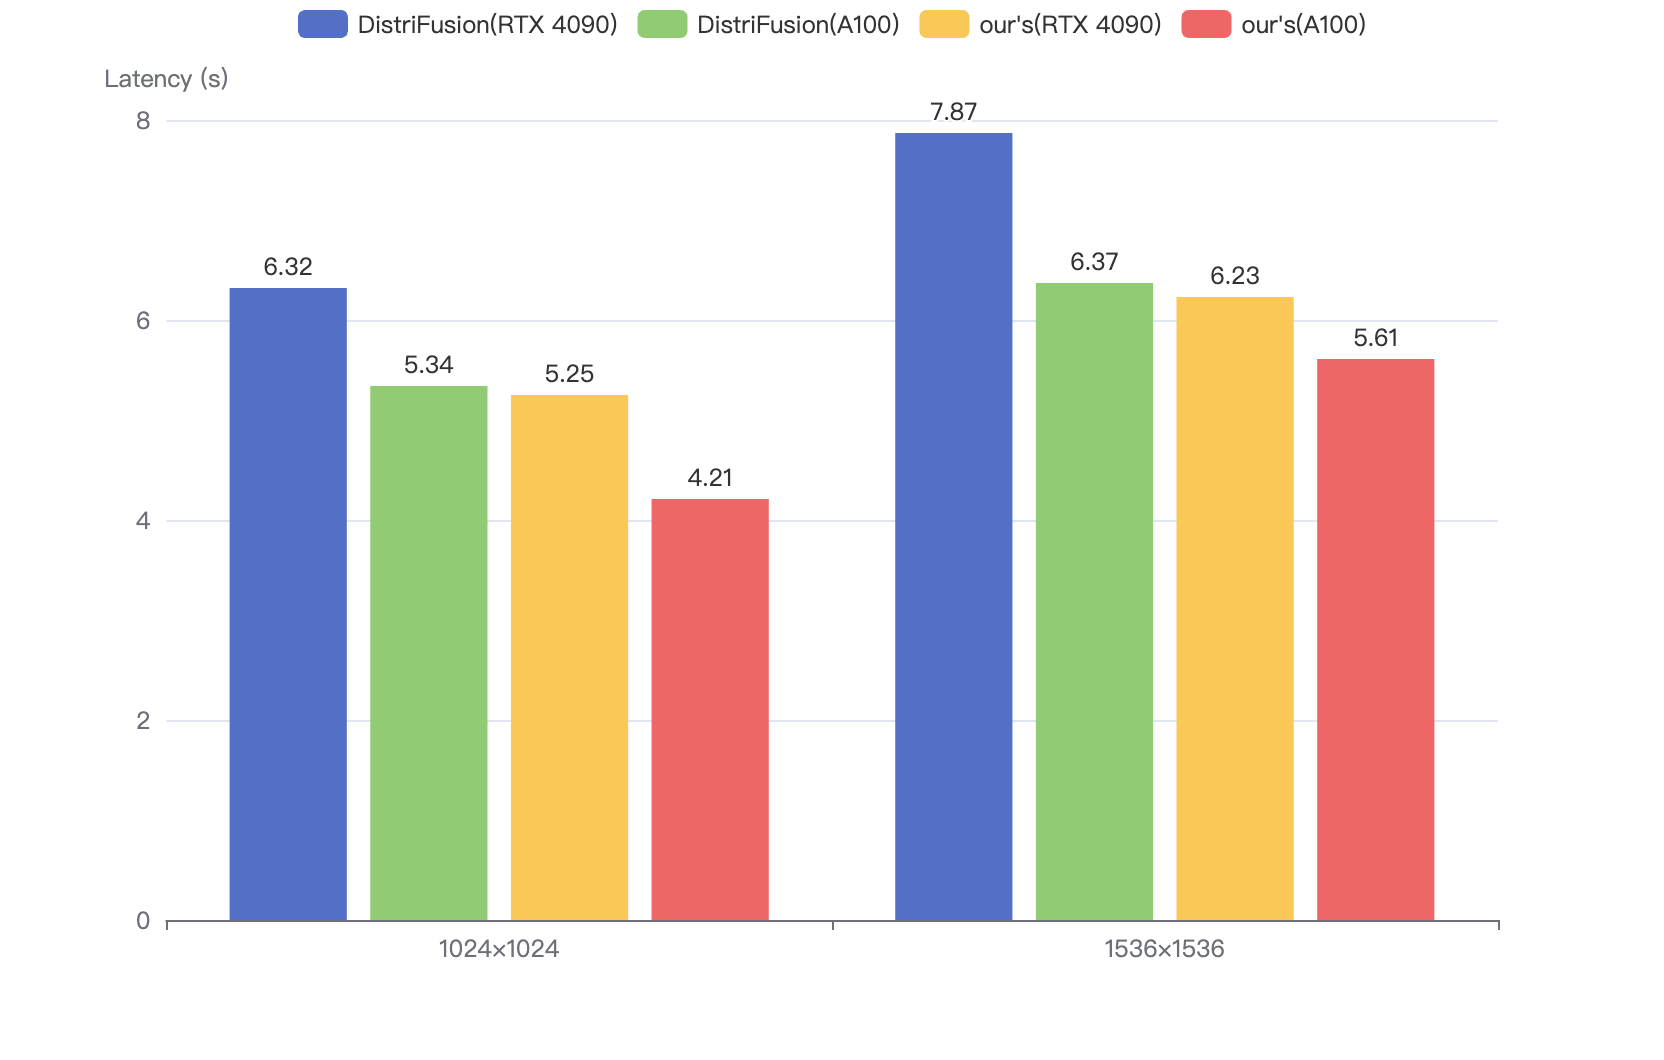
\includegraphics[width=0.8\linewidth]{experiment-result-a100.png}
    \caption{不同GPU阵列及分辨率下本文优化方法与Distrifusion框架的推理性能对比}
    \label{fig:experiment-result-a100}
\end{figure}
\par
分析数据可知,在 RTX 4090 GPU 上,本文优化方法展现出显著的性能优势,
在A100 GPU 性能提升较少,但仍有优势。在低成本的 RTX 4090 上的性能提升更凸显了本文优化方法对于降低分布
式推理框架成本的重要意义 —— 使用成本更低的 RTX 4090 GPU 即可实现更优的推理性能,避免了对高成本 A100 GPU 
及NVLink 技术的依赖,
为扩散模型分布式推理框架在实际应用中降低成本提供了有力支持。

\subsubsection{更高分辨率下的推理运行情况}
除了在 1024×1024 和 1536×1536 分辨率下测试 Stable Diffusion 模型之外,我们还进一步评估了各方法在 
2048×2048 超高分辨率下的推理性能。实验结果(实验环境参见 \autoref{sec:exp-env})表明,在生成 2048×2048 
分辨率图像时,使用 Distrifusion 框架出现了显存不足的问题,导致程序中断;
而采用本文提出的优化方法则能够顺利完成推理任务,没有出现显存溢出情况。
如 \autoref{fig:exp-result-2048} 所示,这表明在高分辨率场景下,本文方法显存管理能力更好。
因此,在面对大规模、高分辨率生成任务时,我们的优化方法在资源效率使用和运行稳定性方面展现出明显优势。
\begin{table}[ht]
    \begin{tabularx}{\linewidth}{
        |l|
        >{\centering\arraybackslash}X|
        >{\centering\arraybackslash}X|
        >{\centering\arraybackslash}X|
        }
        \hline
         & 1024×1024 & 1536×1536 & 2048×2048 \\ \hline
        Distrifusion & \checkmark & \checkmark & × \\ \hline
        Our's & \checkmark & \checkmark & \checkmark \\ \hline
    \end{tabularx}
    \caption{\label{fig:exp-result-2048}Distrifusion框架与本文优化方法在\autoref{sec:exp-env}实验环境下支持生成的图片分辨率对比}
\end{table}
\subsubsection{消融实验}
为验证各模块对扩散模型分布式推理的优化效果,本节基于
第 \ref{sec:communication_freeze_and_async_communication_module_design} 节设计的通信管理模块,
通过控制变量法开展以下消融实验:

\begin{itemize}
\item \textbf{通信冻结模块测试}:在8GPU环境下独立启用该模块,通过冻结层选择器动态调控通信量。
如图 \ref{fig:communication-freeze-module-result} 所示,针对1024×1024及1536×1536分辨率图像生成任务,
相较于原始DistriFusion框架,通信总量降低25\% \~{} 34\%。测试结果显示,该模块通过减少关键路径上的数据传输,
显著降低了整体通信量。
\begin{figure}[ht]
\centering
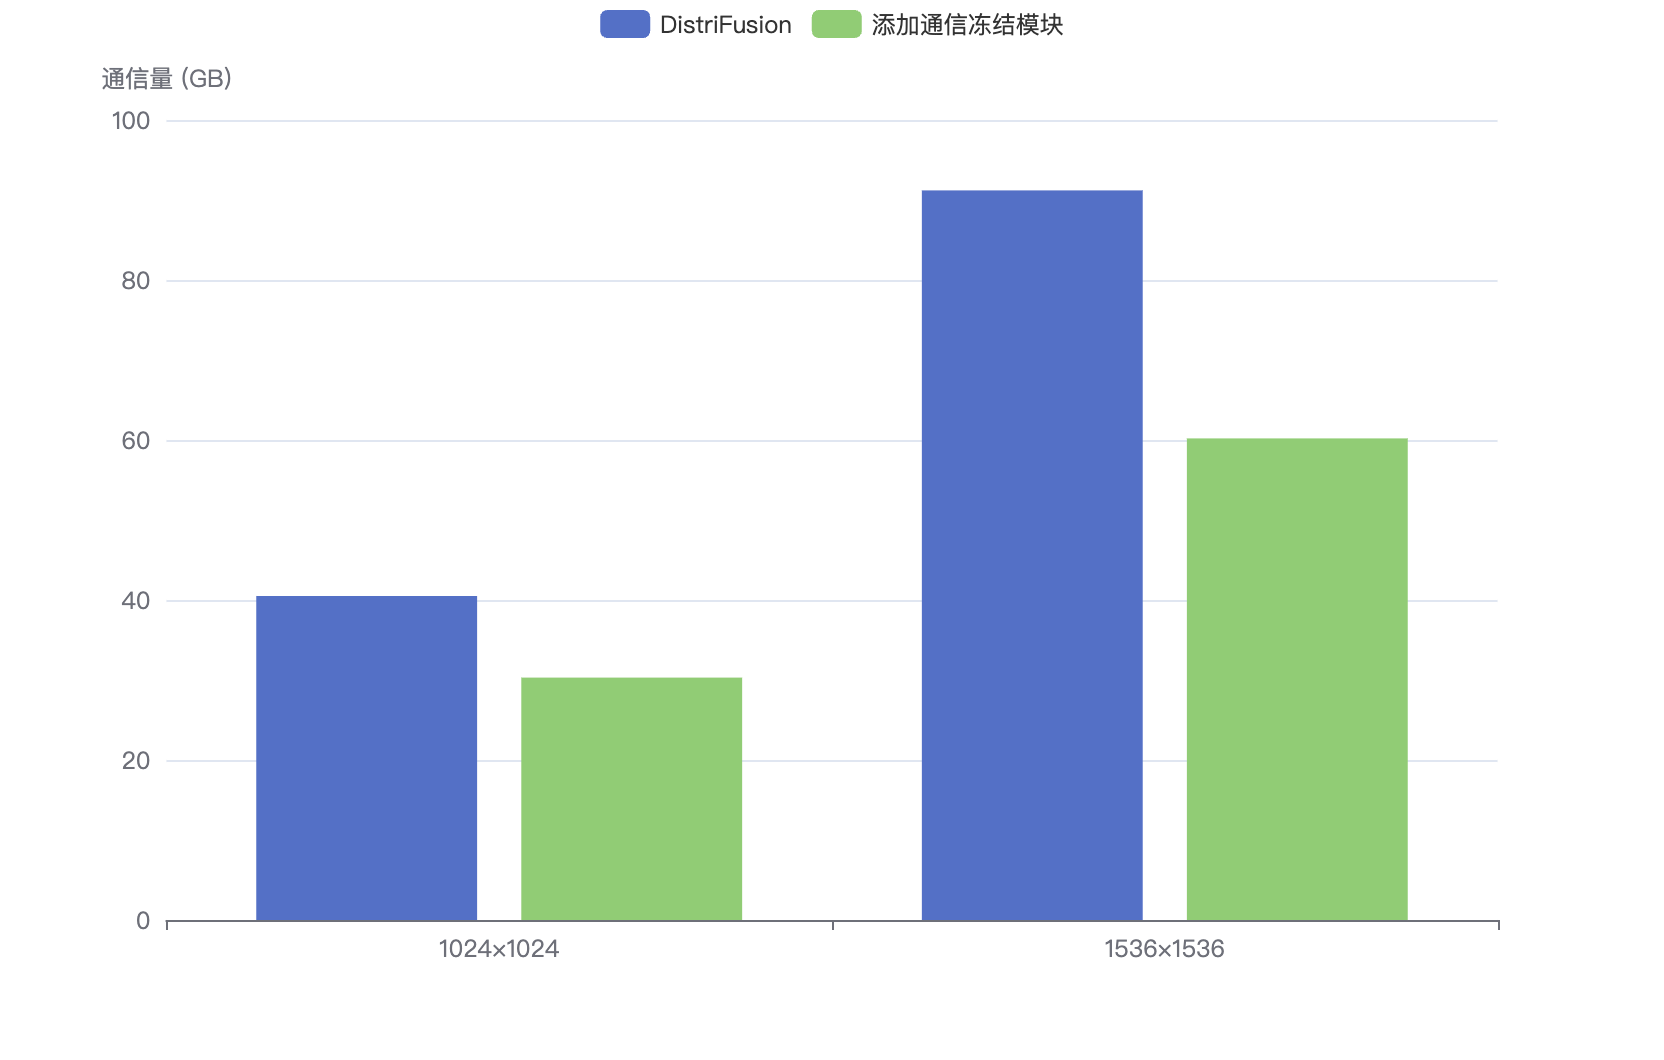
\includegraphics[width=0.7\linewidth]{communication-freeze-module-result.png}
\caption{不同分辨率下通信冻结模块与DistriFusion框架的通信总量对比}
\label{fig:communication-freeze-module-result}
\end{figure}

\item \textbf{异步通信模块测试}:在8GPU配置下独立启用异步通信模块,利用数据块处理器进行细粒度划分,
并通过数据传输管理器优化调度策略。如图 \ref{fig:async-communication-module-result} 所示,
针对相同分辨率的任务,通信时间较基准框架下降约32\%。测试结果显示,
该模块通过异步数据传输有效缩短了通信阶段耗时。
\begin{figure}[ht]
\centering
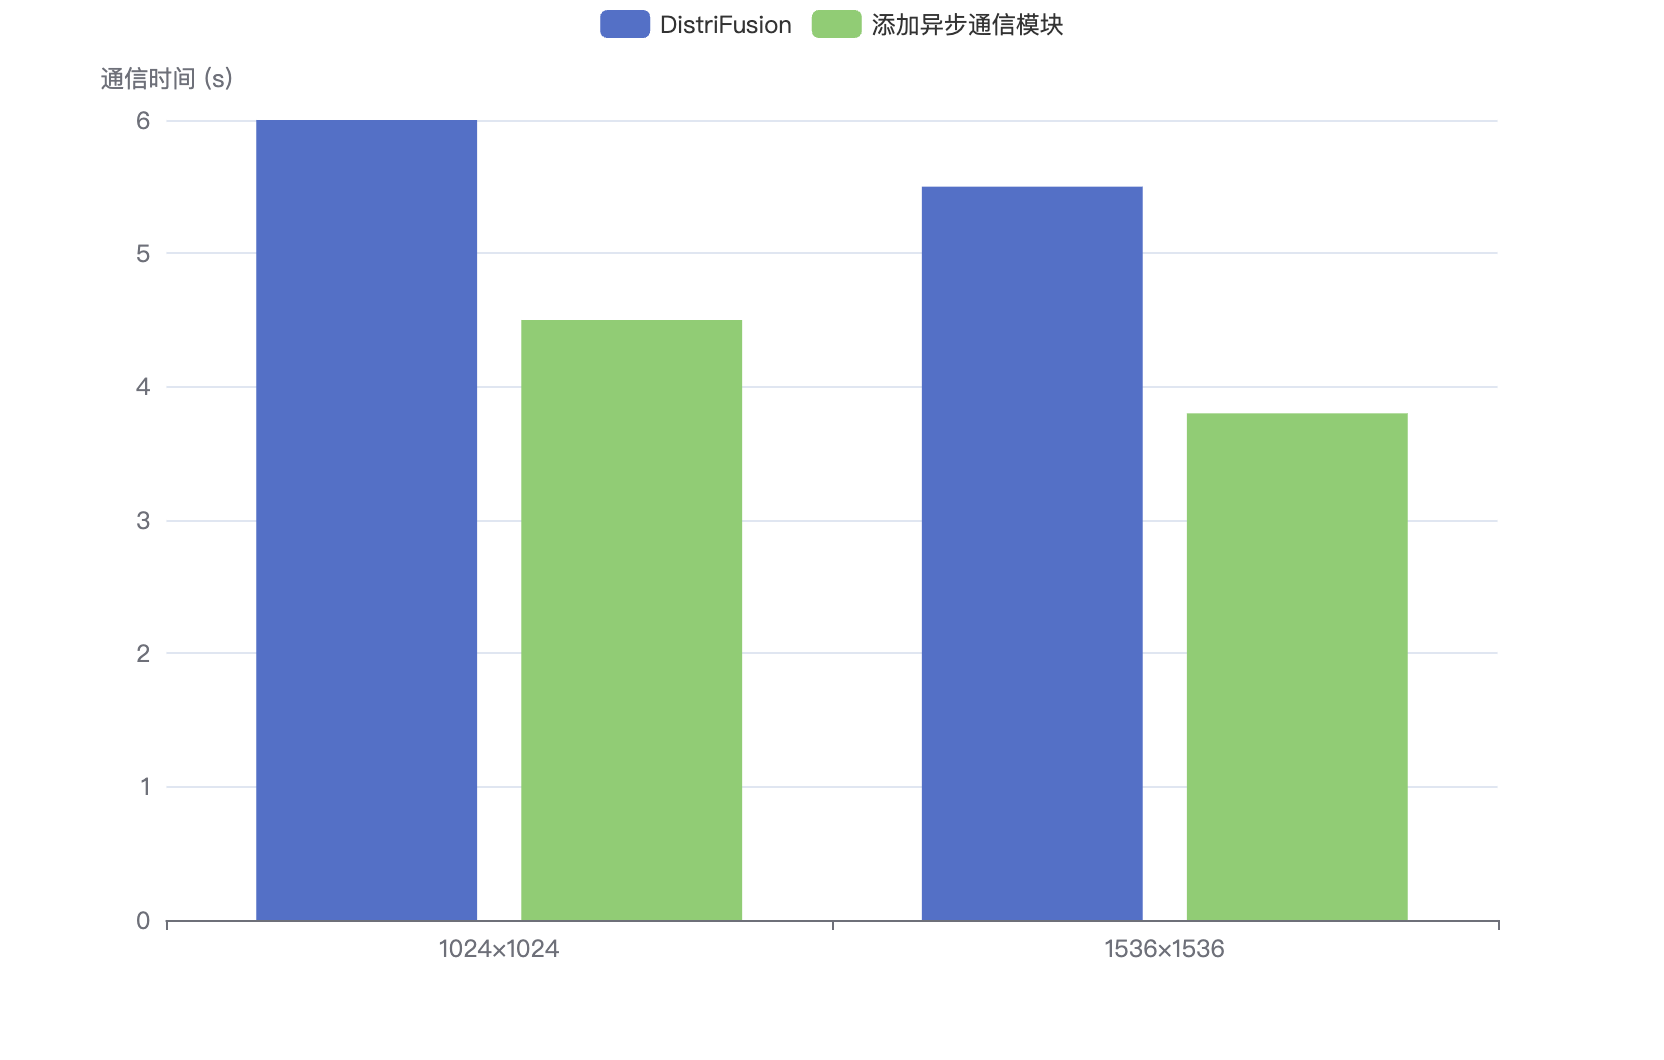
\includegraphics[width=0.7\linewidth]{async-communication-module-result.png}
\caption{不同分辨率下异步通信模块与DistriFusion框架的通信时间对比}
\label{fig:async-communication-module-result}
\end{figure}

\item \textbf{联合影响测试}:在4GPU配置下测试双模块协同效应。
如图 \ref{fig:communication-freeze-and-async-communication-module-result} 所示,
针对1024×1024及1536×1536分辨率任务,添加通信冻结模块后推理延迟降低23\%,叠加异步通信模块后进一步下降10\%。
实验表明双模块具有良好的协同增益。
\begin{figure}[ht]
\centering
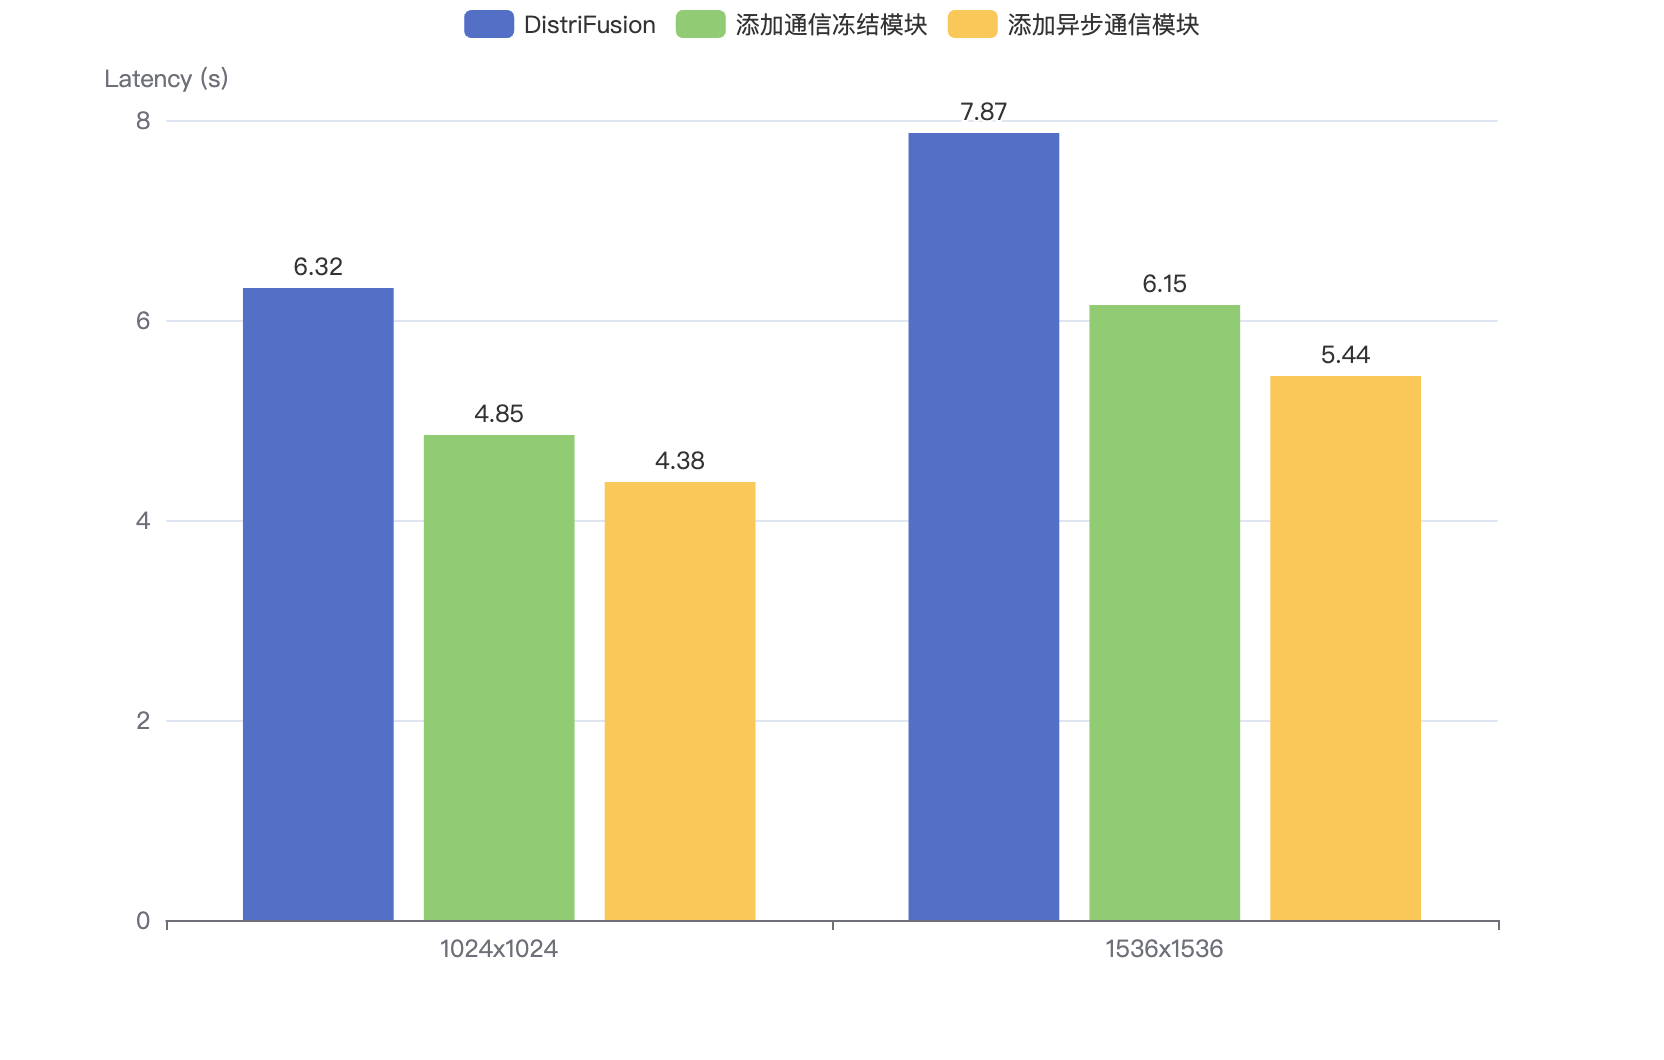
\includegraphics[width=0.8\linewidth]{communication-freeze-and-async-communication-module-result.png}
\caption{双模块协同优化下的推理延迟对比}
\label{fig:communication-freeze-and-async-communication-module-result}
\end{figure}
\end{itemize}
\par
通过系统化的消融实验验证,实验结果表明本文的优化框架不仅实现了通信开销的有效控制,
更通过模块间的协同优化提升了分布式扩散模型的推理效率。这种层次化的优化策略为扩散模型的分布式部署提供了
可扩展的解决方案,具有显著的工程价值。

\section{总结与展望}
\subsection{研究成果总结}
本文围绕扩散模型分布式推理中的通信瓶颈问题,提出了基于通信冻结与异步通信的协同优化框架。通过系统性实验验证,主要成果如下:
\begin{itemize}
    \item \textbf{通信瓶颈量化分析}:在RTX 4090低带宽集群中,DistriFusion框架的通信延迟占比达30\%\~{}40\%
    (如\autoref{fig:communication-delay-1024}所示),显著制约多卡推理性能;
    \item \textbf{优化框架有效性}:本文方法在1024×1024分辨率下,相比基础框架推理延迟降低28\%\~{}43\%,
    且图像质量与DistriFusion相似(如\autoref{tab:image-quality-result}所示);
    \item \textbf{模块协同增益}:通信冻结模块降低通信总量25\%\~{}34\%,异步通信模块进一步缩短通信时间32\%,
    双模块协同实现延迟降低33\%(如\autoref{fig:communication-freeze-and-async-communication-module-result}
    所示)。
\end{itemize}
因此,本文优化框架突破了传统扩散模型分布式推理的高带宽硬件限制,为消费级GPU集群部署(如RTX 4090)提供了可行路径。

\subsection{实验局限性分析}
本研究在通信机制设计中仍存在以下不足:
当前框架主要依赖All-Gather通信(如\autoref{fig:All-Gather}所示),需要将各GPU的全部数据进行通信,
而在基础设想中,对于不同GPU的数据进行详细分析,使用特定GPU进行传输可以进一步减小通信量,但这种设想需要使用
Broadcast方法,而Broadcast方法在具体运行中对数据的储存位置有特点要求,经反复实验,无法使用Broadcast方法进行上述处理,
因此本文通信机制还可以进一步优化\cite{PytorchDistributedDataParallel}。
   

\subsection{未来研究方向}
\begin{itemize}
    \item \textbf{通信模式优化}:目前的优化框架只使用了单一的通信方法,在后续研究下可以
    根据不同计算阶段需求使用不同的通信方式,如在数据同步阶段采用broadcast部分传输,
    在结果整合阶段使用All-Gather传输,从而进一步优化通信效率;
    \item \textbf{优先级通信控制}:在数据通信时,目前的方法对不同数据的传输采取相同的优先级处理,在未来的研究中可以
    进一步开发能自动识别数据重要性来细致化处理不同数据通信的机制,
    在保证生成质量的前提下动态压缩通信数据,提高整体生成质量和推理性能\cite{Ouyang2020CommunicationOS};
    \item \textbf{多模型扩展}:将本优化框架进行扩展,针对其他扩散模型或者其他种类模型设计通用的分布式推理机制
    
\end{itemize}
% \par 我们可以用includegraphics来插入现有的jpg等格式的图片,如\autoref{fig:zju-logo}。

% \begin{figure}[ht]
%     \centering
%     
\includegraphics[width=.4\linewidth]{logo/zju}
%     \caption{\label{fig:zju-logo}浙江大学LOGO}
% \end{figure}

% \par 如\autoref{tab:sample}所示,这是一张自动调节列宽的表格。

% \begin{table}[ht]
%     \caption{\label{tab:sample}自动调节列宽的表格}
%     \begin{tabularx}{\linewidth}{|c|X<{\centering}|}
%         \hline
%         第一列 & 第二列 \\ \hline
%         xxx & xxx \\ \hline
%         xxx & xxx \\ \hline
%         xxx & xxx \\ \hline
%     \end{tabularx}
% \end{table}

% \par 如\autoref{equ:sample},这是一个公式

% \begin{equation}
%     \label{equ:sample}
%     A=\overbrace{(a+b+c)+\underbrace{i(d+e+f)}_{\text{虚数}}}^{\text{复数}}
% \end{equation}

% \par 如\autoref{code:sample}所示,这是一段代码。
% 计算机学院的代码样式可能与其他专业不同,
% 如有需要,可以从计算机学院专业模板中复制相关的代码样式设定。

% \begin{lstlisting}[%
%     language={C},
%     caption={simple.c},
%     label={code:sample}
% ]
% #include <stdio.h>

% int main(int argc, char *argv[])
% {
%     printf("Hello, zjuthesis\n");
%     return 0;
% }
% \end{lstlisting}

% \subsection{关于字体}

% 英文字体通常提供了粗体和斜体的组合,中文字体通常没有粗体或斜体,本模板使用了 `AutoFakeBold' 来实现中文伪粗体,但不提供中文斜体,如\autoref{tab:font-examples}所示。

% \begin{table}
%     \centering
%     \caption{一些字体示例}
%     \label{tab:font-examples}
%     \begin{tabular}{|c|c|c|c|c|}
%         \hline
%         字体            & 常规             & 粗体                       & 斜体                      & 粗斜体                                \\ \hline
%         Times New Roman & Regular         & {\bfseries          Bold} & {\itshape         Italic} & {\bfseries \itshape      BoldItalic} \\ \hline
%         仿宋            & {\fangsong 常规} & {\fangsong \bfseries 粗体} & {\fangsong \itshape 斜体} & {\fangsong \bfseries \itshape 粗斜体} \\ \hline
%         宋体            & {\songti   常规} & {\songti   \bfseries 粗体} & {\songti   \itshape 斜体} & {\songti   \bfseries \itshape 粗斜体} \\ \hline
%         黑体            & {\heiti    常规} & {\heiti    \bfseries 粗体} & {\heiti    \itshape 斜体} & {\heiti    \bfseries \itshape 粗斜体} \\ \hline
%         楷体            & {\kaishu   常规} & {\kaishu   \bfseries 粗体} & {\kaishu   \itshape 斜体} & {\kaishu   \bfseries \itshape 粗斜体} \\ \hline
%     \end{tabular}
% \end{table}

% \sectionnonum[none]{同一页上的章标题}
